\chapter{ORIUS Framework and Theoretical Foundations}
\label{ch:ch04_theoretical_foundations}
\label{ch:mathematical-foundations}

% --- Merged from ch09_dc3s_battery_adapter.tex ---

\section{DC3S: The Universal Safety Adapter}
\label{ch:dc3s-adapter}
\label{ch:dc3s}

The Detect--Calibrate--Constrain--Shield--Certify Safety System (DC3S) is the
runtime adapter that sits at the Optimize--Dispatch boundary
(Chapter~\ref{ch:orius-context}) and translates degraded observations
into safety-guaranteed actions.  This chapter specifies the runtime objects,
derives each stage of the pipeline, and narrates a complete control step from
telemetry ingestion to certificate issuance.

In the codebase, the domain-agnostic version of that runtime now lives in
\path{src/orius/universal_theory/}.  The battery derivation below is the
reference instantiation of that universal degraded-observation kernel, not a
hidden claim that every domain already inherits battery-level proof depth.

% ----------------------------------------------------------------
\subsection{Why a Runtime Shield Is Needed}

Chapter~\ref{ch:forecasting} showed that CQR intervals under-cover
conditionally: wind coverage drops to 39--49\% in the low-reliability group,
and load coverage falls 8--20 percentage points below nominal.  A dispatch
controller that trusts these intervals without adjustment will issue actions
that violate SOC constraints on the true (unobserved) trajectory at rates far
exceeding the design budget~$\alpha$.

A runtime shield is needed because:
\begin{enumerate}
  \item Forecast calibration is a \emph{batch} property; telemetry degradation
    is a \emph{streaming} property.  No static calibration fold can anticipate
    the specific fault pattern at step~$t$.
  \item The observation quality at step~$t$ is \emph{known} to the controller
    (via packet-loss counters, staleness timers, and drift detectors) but is
    \emph{not used} by standard conformal methods.
  \item The SOC dynamics are \emph{coupled}: an unsafe action at $t$ may
    render all future actions infeasible.  The shield must prevent the
    first violation, not merely reduce its frequency.
\end{enumerate}

% ----------------------------------------------------------------
\subsection{Runtime Objects}
\label{sec:runtime-objects}

Table~\ref{tab:runtime-objects} defines the variables maintained by DC3S at
each control step.

\begin{table}[ht]
\centering
\caption{DC3S runtime objects at step~$t$.}
\label{tab:runtime-objects}
\begin{tabular}{cll}
\toprule
\textbf{Symbol} & \textbf{Name} & \textbf{Description} \\
\midrule
$z_t$            & True state          & Actual plant state (load, renew., SOC);
                                         unobserved at runtime \\
$\tilde{z}_t$    & Observed state      & Telemetry-degraded plant state seen by
                                         controller \\
$o_t$            & Observation vector  & Raw sensor packet (may contain NaN,
                                         delays, spikes) \\
$x_t$            & Feature vector      & Engineered features derived from
                                         $\tilde{z}_{1:t}$ \\
$w_t$            & Reliability score   & $\in [0,1]$; OQE output quantifying
                                         observation quality \\
$d_t$            & Drift flag          & $\in \{0,1\}$; Page--Hinkley detector
                                         output \\
$s_t$            & Stale count         & Non-negative integer; consecutive steps
                                         since last fresh reading \\
$C_t(\alpha)$    & Base interval       & CQR prediction interval at
                                         miscoverage~$\alpha$ \\
$C_t^{\mathrm{RAC}}(\alpha)$ & Inflated interval &
                   Reliability-adaptive conformal interval \\
$\mathcal{A}_t$  & Safe-action set     & Feasible actions under inflated
                                         uncertainty \\
$a_t^\star$      & Candidate action    & Optimiser output \\
$a_t^{\mathrm{safe}}$ & Safe action    & Projected action $\in \mathcal{A}_t$ \\
$\mathcal{C}_t$  & Certificate         & Step-level audit record \\
\bottomrule
\end{tabular}
\end{table}

% ----------------------------------------------------------------
\subsection{Detect: Telemetry Reliability Scoring (OQE)}
\label{sec:detect}

The Observation Quality Estimator (OQE) computes the reliability score
$w_t \in [0, 1]$ from three sub-scores:

\begin{equation}
\label{eq:oqe}
  w_t = w_t^{\mathrm{fresh}} \cdot w_t^{\mathrm{range}} \cdot w_t^{\mathrm{consist}},
\end{equation}
where:
\begin{description}
  \item[$w_t^{\mathrm{fresh}}$] Freshness score: $\exp(-\lambda_f \cdot s_t)$,
    decaying exponentially with the stale count~$s_t$.
  \item[$w_t^{\mathrm{range}}$] Range plausibility: 1 if all channels are
    within physical bounds, decayed proportionally to the number of
    out-of-range channels.
  \item[$w_t^{\mathrm{consist}}$] Temporal consistency: based on the
    Mahalanobis distance of the current reading from a short rolling window,
    penalising spikes and discontinuities.
\end{description}

The OQE computation is stateless given the rolling buffer and runs in
$<0.03$\,ms median latency
(Table~\ref{tab:dc3s-latency}, \texttt{reports/publication/dc3s\_latency\_summary.csv}).

% ----------------------------------------------------------------
\subsection{Calibrate: Reliability-Adaptive Interval Inflation}
\label{sec:calibrate}

The base CQR interval $C_t(\alpha)$ is inflated to compensate for the
conditional under-coverage revealed in Chapter~\ref{ch:forecasting}.  The
\emph{RAC-Cert} (Reliability-Adaptive Conformal Certificate) formula is:

\begin{equation}
\label{eq:rac-cert}
\boxed{
  C_t^{\mathrm{RAC}}(\alpha) \;=\;
  C_t(\alpha) \;\cdot\;
  \bigl[\,1 + \kappa_r\,(1 - w_t)
             + \kappa_d\,d_t
             + \kappa_s\,s_t\,\bigr]
}
\end{equation}

where:
\begin{description}
  \item[$\kappa_r$] Reliability sensitivity: scales the inflation with the
    complement of the reliability score.  Default $\kappa_r = 0.5$.
  \item[$\kappa_d$] Drift sensitivity: additive inflation when the
    Page--Hinkley detector fires.  Default $\kappa_d = 0.3$.
  \item[$\kappa_s$] Staleness sensitivity: linear inflation per stale step.
    Default $\kappa_s = 0.05$.
\end{description}

The multiplicative form ensures that under nominal conditions
($w_t = 1$, $d_t = 0$, $s_t = 0$) the inflated interval collapses to the
base interval, imposing zero additional conservatism.

\paragraph{Inflation diagnostics.}
The locked evidence in \texttt{reports/publication/dc3s\_main\_table.csv}
reports the mean and P95 of the RAC inflation factor across all scenarios
and seeds.  Under the \texttt{drift\_combo} scenario the mean inflation
is approximately $1.02$, rising to $1.05$ at the P95 level, confirming that
the adaptive layer adds modest width only when observation quality genuinely
degrades.

% ----------------------------------------------------------------
\subsection{Constrain: Safe-Action Sets Under Widened Uncertainty}
\label{sec:constrain}

Given the inflated interval $C_t^{\mathrm{RAC}}(\alpha)$ with half-width
$q_t^{\mathrm{RAC}}$, the safe-action set is constructed by tightening
the SOC bounds (cf.\ Equation~\eqref{eq:tightened-bounds},
Chapter~\ref{ch:battery-dynamics}):

\begin{equation}
\label{eq:safe-action-set}
  \mathcal{A}_t = \Bigl\{\,(P^{+}, P^{-}) \;\Big|\;
    E_{\min} + q_t^{\mathrm{RAC}} \;\le\; \hat{E}_{t+1}(P^{+}, P^{-})
    \;\le\; E_{\max} - q_t^{\mathrm{RAC}},\;
    \text{power and ramp constraints hold}\,\Bigr\},
\end{equation}
where $\hat{E}_{t+1}(P^{+}, P^{-})$ is the one-step-ahead SOC estimate
under the candidate action and the observed initial SOC~$\tilde{E}_t$.

If $q_t^{\mathrm{RAC}}$ is large enough that $\mathcal{A}_t = \emptyset$,
the controller reverts to a safe-standby action
$(P^{+} = 0, P^{-} = 0)$, which is always feasible.

% ----------------------------------------------------------------
\subsection{Shield: Projection and Repair}
\label{sec:shield}

If the candidate action $a_t^\star$ lies outside $\mathcal{A}_t$, the shield
projects it to the nearest safe action:

\begin{equation}
\label{eq:repair}
\boxed{
  a_t^{\mathrm{safe}} = \argmin_{a \in \mathcal{A}_t}
    \|a - a_t^\star\|_2
}
\end{equation}

Because $\mathcal{A}_t$ is a convex polytope (intersection of linear
half-spaces from power bounds, ramp limits, and tightened SOC bounds), the
projection is a quadratic programme solvable in closed form for the
single-step case or via an efficient QP solver for the multi-step horizon.

The \emph{intervention rate} (IR) is the fraction of steps where
$a_t^{\mathrm{safe}} \neq a_t^\star$:
\[
  \mathrm{IR} = \frac{1}{T} \sum_{t=1}^{T}
    \mathbf{1}\!\bigl[a_t^{\mathrm{safe}} \neq a_t^\star\bigr].
\]

The locked benchmark results show that DC3S achieves IR~$\approx 2{-}8\%$
under degraded scenarios while maintaining TSVR~$= 0\%$, confirming that the
economic cost of safety is modest.

% ----------------------------------------------------------------
\subsection{FTIT State Tube}
\label{sec:ftit}

The Fault-Tolerant Invariant Tube (FTIT) provides a secondary safety layer
that does not depend on interval calibration.  FTIT propagates worst-case
SOC bounds forward over a $k$-step horizon:

\begin{equation}
\label{eq:ftit}
\begin{aligned}
  \overline{E}_{t+k} &= \hat{E}_t + \delta_{\max}
    + k\,\eta^{+}\,P_{\max}^{+}\,\Delta t, \\
  \underline{E}_{t+k} &= \hat{E}_t - \delta_{\max}
    - k\,P_{\max}^{-}/\eta^{-}\,\Delta t,
\end{aligned}
\end{equation}
where $\delta_{\max}$ is the maximum SOC estimation error consistent with
the current reliability score.  Any action that would cause either bound to
exit $[E_{\min}, E_{\max}]$ within the $k$-step tube is rejected.

The FTIT acts as a hard backstop: even if the RAC-Cert inflation is
insufficient (e.g.\ due to a novel fault type not captured by the
sensitivity parameters), the tube prevents multi-step SOC excursions.

% ----------------------------------------------------------------
\subsection{Certify: Step-Level Audit Records}
\label{sec:certify}

At the conclusion of each control step, DC3S emits a certificate
$\mathcal{C}_t$ containing:

\begin{table}[ht]
\centering
\caption{DC3S certificate fields.}
\label{tab:certificate-fields}
\begin{tabular}{ll}
\toprule
\textbf{Field} & \textbf{Content} \\
\midrule
\texttt{step}                    & Time-step index \\
\texttt{timestamp}               & UTC timestamp \\
\texttt{reliability\_w}          & Observation quality score $w_t$ \\
\texttt{drift\_flag}             & Page--Hinkley drift indicator $d_t$ \\
\texttt{inflation}               & RAC-Cert multiplier \\
\texttt{proposed\_charge\_mw}    & Candidate charge power $P_t^{+\star}$ \\
\texttt{proposed\_discharge\_mw} & Candidate discharge power $P_t^{-\star}$ \\
\texttt{safe\_charge\_mw}        & Repaired charge power \\
\texttt{safe\_discharge\_mw}     & Repaired discharge power \\
\texttt{intervened}              & Boolean: was the action repaired? \\
\texttt{intervention\_reason}    & Reason string (SOC, ramp, BMS) \\
\texttt{guarantee\_passed}       & Boolean: all invariants satisfied? \\
\texttt{soc\_after\_mwh}         & Estimated SOC after action \\
\bottomrule
\end{tabular}
\end{table}

A trace of certificate records for a representative episode is stored in
\texttt{reports/publication/dc3s\_step\_trace.csv}.  The certificate
stream is the primary input to the monitoring stage
(Chapter~\ref{ch:orius-context}) and to the half-life analysis
(Chapter~\ref{ch:cert-half-life-blackout}).

% ----------------------------------------------------------------
\subsection{DC3S Latency Profile}

Real-time dispatch requires that the DC3S pipeline complete within the
control cycle (typically 1\,s for sub-hourly, 60\,s for hourly).
Table~\ref{tab:dc3s-latency} reports the component-level latency from the
locked benchmark.

\begin{table}[ht]
\centering
\caption{DC3S component latency (ms).  Source:
\texttt{reports/publication/dc3s\_latency\_summary.csv}.}
\label{tab:dc3s-latency}
\begin{tabular}{lrrrrr}
\toprule
\textbf{Component} & \textbf{Mean} & \textbf{Median} & \textbf{P95} &
  \textbf{P99} & \textbf{Max} \\
\midrule
Reliability scoring          & 0.026 & 0.021 & 0.043 & 0.130 & 0.712 \\
Drift update (Page--Hinkley) & 0.000 & 0.000 & 0.001 & 0.001 & 0.160 \\
Uncertainty set build        & 0.012 & 0.011 & 0.011 & 0.047 & 0.724 \\
Action repair (projection)   & 0.002 & 0.002 & 0.002 & 0.003 & 0.210 \\
\midrule
\textbf{Full DC3S step}      & 0.042 & 0.037 & 0.041 & 0.193 & 2.416 \\
\bottomrule
\end{tabular}
\end{table}

The full DC3S step completes in under 0.2\,ms at P99, well within the
budget for any practical control cycle.  The maximum of 2.4\,ms occurs
during JIT warm-up on the first step and is not representative of
steady-state performance.

% ----------------------------------------------------------------
\subsection{Complete Runtime Narrative}
\label{sec:runtime-narrative}

A single DC3S control step proceeds as follows:

\begin{enumerate}
  \item \textbf{Receive observation} $o_t$ from the telemetry gateway.
    If the packet is missing (dropout), carry forward the last valid reading
    and increment~$s_t$.

  \item \textbf{Detect.}  Compute $w_t = w_t^{\mathrm{fresh}} \cdot
    w_t^{\mathrm{range}} \cdot w_t^{\mathrm{consist}}$ via OQE.
    Run the Page--Hinkley test on the residual stream to set~$d_t$.

  \item \textbf{Calibrate.}  Inflate the base CQR interval:
    $C_t^{\mathrm{RAC}}(\alpha) = C_t(\alpha) \cdot
    [1 + \kappa_r(1-w_t) + \kappa_d\,d_t + \kappa_s\,s_t]$.

  \item \textbf{Constrain.}  Construct the safe-action set $\mathcal{A}_t$
    by tightening SOC bounds with the inflated half-width.  Verify the
    FTIT tube; if the tube is violated, further restrict $\mathcal{A}_t$.

  \item \textbf{Shield.}  If $a_t^\star \notin \mathcal{A}_t$, project:
    $a_t^{\mathrm{safe}} = \argmin_{a \in \mathcal{A}_t} \|a - a_t^\star\|_2$.
    Otherwise $a_t^{\mathrm{safe}} = a_t^\star$.

  \item \textbf{Certify.}  Emit the certificate $\mathcal{C}_t$ recording
    all runtime variables, the intervention decision, and the
    guarantee-check outcome.  Forward $a_t^{\mathrm{safe}}$ to the BMS.
\end{enumerate}

% ----------------------------------------------------------------
\subsection{Chapter Summary}

This chapter specified the DC3S battery adapter: a five-stage runtime shield
(Detect, Calibrate, Constrain, Shield, Certify) that intercepts dispatch
actions at the Optimize--Dispatch boundary.  The OQE reliability
scorer~\eqref{eq:oqe} quantifies observation quality; the RAC-Cert
formula~\eqref{eq:rac-cert} inflates intervals adaptively; the safe-action
set~\eqref{eq:safe-action-set} tightens SOC bounds accordingly; and the
projection repair~\eqref{eq:repair} moves unsafe actions to the nearest
feasible point.  The FTIT tube provides a calibration-free safety backstop.
The full pipeline completes in under 0.2\,ms at P99, and step-level
certificates create a complete audit trail.  Empirical validation is
presented in Chapter~\ref{ch:cpsbench}.


% --- Merged from ch15_assumptions_notation_proof_discipline.tex ---

\section{Assumptions, Notation, and Proof Discipline}
\label{ch:assumptions}

This chapter establishes the formal scaffolding for Part~III.  It fixes
notation that is stable across all theorems, catalogues the eight
standing assumptions, defines the proof dependency matrix, and sets the
disciplinary standards that every subsequent proof must satisfy.  The
flagship DC3S ladder in Chapters~\ref{ch:theorem-oasg}--\ref{ch:temporal-extensions}
contains eight principal theorems (T1--T8), but it is not the entire theorem
surface of the dissertation.  The live master-manuscript include tree now
contains additional theorem-carrying merged chapters, appendix restatements,
and front-loaded formal definitions.  The audited surface therefore contains
\textbf{83 formal items} (26~theorems, 5~lemmas, 9~propositions,
12~corollaries, 15~definitions, 16~assumptions), all audited in
Appendix~\ref{app:integrated-theorem-surface-register} and summarised in
Table~\ref{tab:integrated-theorem-surface-summary} at the end of this chapter.

\subsection{Stable Notation}

Throughout Part~III, the following symbols have fixed meaning:

\begin{center}
\begin{tabular}{cl}
\toprule
\textbf{Symbol} & \textbf{Meaning} \\
\midrule
$x_t$ & True (plant-internal) state at step $t$ \\
$\hat{x}_t$ & Observed (telemetry-delivered) state at step $t$ \\
$a_t$ & Action (dispatch decision) at step $t$ \\
$\phi(x_t)$ & Safety predicate: $\phi(x_t) = 1$ iff $x_t$ satisfies all constraints \\
$w_t$ & Reliability score, $w_t \in [0,1]$ \\
$\alpha$ & Conformal miscoverage level (nominal $\alpha = 0.10$) \\
$q_t$ & Conformal quantile (half-width of the prediction interval) \\
$\mathcal{A}_t$ & Tightened safe-action set at step $t$ \\
$T$ & Episode horizon (number of steps) \\
$V$ & Total violation count: $V = \sum_{t=1}^T \mathbf{1}[\lnot\,\phi(x_t)]$ \\
$\bar{w}$ & Episode-average reliability: $\bar{w} = T^{-1}\sum_t w_t$ \\
\bottomrule
\end{tabular}
\end{center}

\paragraph{Semantics of the reliability score.}
The symbol $w_t$ is treated throughout this dissertation as a
\emph{runtime reliability score}, not as a probability by definition.
It records how trustworthy the telemetry channel appears at step $t$
according to the OQE pipeline and adjacent runtime checks.  A theorem may
convert $w_t$ into a probabilistic statement only when that conversion is
spelled out explicitly as an extra theorem-local hypothesis.

\paragraph{Battery instantiation.}
In the battery domain, $x_t = \text{SOC}_t$ (MWh),
$a_t = (P_t^{\text{chg}}, P_t^{\text{dis}})$ (MW), and
$\phi(x_t) = \mathbf{1}[\text{SOC}_{\min} \le x_t \le \text{SOC}_{\max}]$.

\subsection{Assumption IDs (A1--A13)}

Each assumption is assigned a permanent identifier and stated in both
domain-general and battery-specific form.

\begin{assumption}[A1: Bounded model error]
\label{assm:A1}
The one-step prediction error $\|x_{t+1} - f(x_t, a_t)\|$ is bounded
by a known constant $\epsilon_{\text{model}}$.
\emph{Battery:} $|x_{t+1} - (x_t + \eta\,P_t\,\Delta t)| \le \epsilon_{\text{model}}$.
\end{assumption}

\begin{assumption}[A2: Bounded telemetry error]
\label{assm:A2}
The observation error $\|\hat{x}_t - x_t\|$ is bounded by a
reliability-dependent function: $\|\hat{x}_t - x_t\| \le g(w_t)$,
where $g$ is monotone decreasing.
\end{assumption}

\begin{assumption}[A3: Feasible safe repair]
\label{assm:A3}
For every state $x_t$ satisfying $\phi(x_t) = 1$, there exists at
least one action $a_t \in \mathcal{A}_t$ such that $\phi(x_{t+1}) = 1$.
\end{assumption}

\begin{assumption}[A4: Known dynamics]
\label{assm:A4}
The transition function $f(x_t, a_t)$ is known to the controller up
to the model error bounded in A1.
\emph{Battery:} the SOC transition $x_{t+1} = x_t + \eta\,P_t\,\Delta t$
is known with efficiency $\eta$ identified offline.
\end{assumption}

\begin{assumption}[A5: Monotone bounded uncertainty inflation]
\label{assm:A5}
The inflation function $\iota(w_t) = q_t / (w_t + \epsilon)$ is
monotone decreasing in $w_t$ and bounded: $\iota(w_t) \le \bar{\iota}$
for all $w_t \in [0,1]$.
\end{assumption}

\begin{assumption}[A6: Bounded detector lag]
\label{assm:A6}
The OQE reliability score $w_t$ reflects each telemetry fault within a
channel-specific lag budget.  If a fault begins at step $t_f$, then the
runtime detector fires or the reliability score crosses the alert threshold
within at most $\tau_{\max}(f)$ steps, with
\[
  \tau_{\max}(\text{dropout}) = 1,\quad
  \tau_{\max}(\text{stale}) = 3,\quad
  \tau_{\max}(\text{delay}) = 2,\quad
  \tau_{\max}(\text{out-of-order}) = 10,\quad
  \tau_{\max}(\text{spike}) = 1,\quad
  \tau_{\max}(\text{drift}) = 48.
\]
These constants are mirrored by the runtime diagnostics in
\texttt{src/orius/dc3s/quality.py} and are intended as the defended detector
contract for the locked replay surfaces.
\end{assumption}

\begin{assumption}[A7: Causal certificate update]
\label{assm:A7}
The certificate $\mathcal{C}_t$ depends only on information available
at or before step $t$: $\mathcal{C}_t = h(\hat{x}_{1:t}, a_{1:t-1})$.
\end{assumption}

\begin{assumption}[A8: Admissible fallback policy]
\label{assm:A8}
There exists a fallback policy $\pi_{\text{fb}}$ such that, starting from a
safe state, the runtime can either safely hold the current state in place or
apply a boundary-aware recovery action that moves the state inward.  If neither
case can be certified, the runtime fails closed instead of claiming a fallback
guarantee.
\emph{Battery:} zero dispatch is the defended hold action on the interior, and
safe landing is the defended boundary-recovery action near the SOC limits.
\end{assumption}

\subsection{Proof Dependency Matrix}

Table~\ref{tab:proof-deps} shows which assumptions each theorem requires.

\begin{table}[htbp]
\centering
\caption{Assumption and local-contract dependencies of the full T1--T11 theorem program.}
\label{tab:proof-deps}
\resizebox{\textwidth}{!}{%
\begin{tabular}{lccccccccccp{4.7cm}}
\toprule
\textbf{Theorem} & \textbf{A1} & \textbf{A2} & \textbf{A3} & \textbf{A4}
  & \textbf{A5} & \textbf{A5$'$} & \textbf{A6} & \textbf{A6$'$}
  & \textbf{A7} & \textbf{A8} & \textbf{Extra local contract or witness} \\
\midrule
T1 OASG Existence & \checkmark & \checkmark & & \checkmark & & & & & & & Boundary-reachability witness near the constraint surface \\
T2 Safety Preservation & \checkmark & \checkmark & \checkmark & \checkmark & \checkmark & & & & \checkmark & & Inflated-set containment plus repair membership in the tightened safe set \\
T3 Core Bound & \checkmark & \checkmark & & \checkmark & \checkmark & & \checkmark & & \checkmark & & Predictable risk-envelope budget $r_t \le \alpha(1-w_t)$ \\
T4 Observation Necessity & & \checkmark & & & & & & & & Fixed-margin, quality-ignorant controller class and admissible degraded-observation witness \\
T5 Certificate Horizon & \checkmark & \checkmark & & \checkmark & \checkmark & & \checkmark & & \checkmark & & Forward-tube containment construction \\
T6 Certificate Expiration Bound & & & & \checkmark & \checkmark & & \checkmark & & \checkmark & & Closed-form first-passage lower bound with explicit confidence parameter \\
T7 Feasible Fallback Existence & \checkmark & & & \checkmark & & & & & & \checkmark & Piecewise hold-or-safe-landing fallback construction \\
T8 Graceful Degradation Dominance & \checkmark & \checkmark & \checkmark & \checkmark & \checkmark & & & & & \checkmark & Shared-fault comparison coupling between graceful and uncontrolled release \\
T9 Universal Impossibility & & & & \checkmark & & & & \checkmark & & & Per-window degraded-observation witness under persistent degradation \\
T10 Boundary-Indistinguishability Lower Bound & \checkmark & \checkmark & & & & \checkmark & & & & & Boundary prior and observation-law indistinguishability hypothesis \\
T11 Typed Structural Transfer & & & & & & & & & & & Coverage, soundness, repair-membership, and fallback-admissibility obligations \\
\bottomrule
\end{tabular}%
}
\end{table}

\noindent\textit{Reading note.}  The first ten columns record standing
assumptions.  The final column records theorem-local contracts or structural
witnesses that are not promoted to global assumptions because they are only
needed for the specific theorem in that row.

\subsection{Marginal Versus Conditional Coverage}

A critical distinction throughout Part~III:
\begin{description}
  \item[Marginal coverage.] $\Pr[\,x_t \in \hat{C}_t\,] \ge 1 - \alpha$
    averaged over the randomness of calibration and test points.
    This is what CQR provides.
  \item[Conditional coverage.] $\Pr[\,x_t \in \hat{C}_t \mid \hat{x}_t\,]
    \ge 1 - \alpha$ for every observed value.  Conditional coverage is
    strictly stronger and is \emph{not} guaranteed by CQR without
    additional distributional assumptions.
\end{description}

The ORIUS theorems are stated under marginal coverage unless a stronger
conditioning statement is written explicitly into the theorem assumptions.
The reference proof ladder uses monotone inflation to preserve the base
coverage surface.  The transfer theorem is kept at the one-step level for
exactly this reason: it does not silently upgrade marginal coverage into a
stronger episode-level conditioning claim.

\subsection{Theorem-Local Calibration Contracts}

Two theorem-local contracts are used repeatedly in the tightened theory
surface:
\begin{enumerate}
  \item \textbf{Risk-envelope contract.}  A chapter may introduce a
    predictable sequence $r_t$ satisfying
    $\Prob[x_{t+1}\notin\mathcal{S}\mid \mathcal{H}_t] \le r_t$.
    The reference-row envelope $r_t \le \alpha(1-w_t)$ is one such
    contract, but it is not claimed to follow from vanilla conformal
    exchangeability alone.
  \item \textbf{Boundary-indistinguishability contract.}  A chapter may
    model degraded observation through pairs of latent hypotheses whose
    observation laws remain close in total variation or another explicit
    channel metric.  This is the extra ingredient used in the stylized
    lower-bound theorem (T10); it is not inherited automatically from the
    definition of $w_t$.
\end{enumerate}

\subsection{One-Step Versus Multi-Step Claims}

The theorems in Chapters~\ref{ch:theorem-oasg}--\ref{ch:core-bound}
operate on a \emph{per-step} basis: each step's safety is analysed
conditionally on the current state.  The core bound
(Chapter~\ref{ch:core-bound}) aggregates per-step risks into an
episode-level expectation via linearity of expectation.

Multi-step claims (certificate horizon, graceful degradation) require
additional assumptions about temporal dependence; these are stated
explicitly in Chapter~\ref{ch:temporal-extensions}.

\subsection{Main Result Arc and Traceability IDs}

The manuscript presents the theory as four flagship theorem roles plus
supporting definitions, propositions, and corollaries, while retaining the
permanent T1--T11 identifiers for auditability, appendix mapping, and code
traceability.  This distinction is deliberate: reviewers should read a compact
argument, while the repository keeps the finer-grained theorem IDs needed for
tests, generated registers, and proof-to-code evidence.

\begin{enumerate}
  \item \textbf{Observation-aware safety gap.}  T1 establishes that degraded
    observation can make observed-state safety disagree with true-state safety.
  \item \textbf{Observation necessity.}  T4 establishes that fixed-margin,
    quality-ignorant release cannot guarantee true-state safety on the defended
    ambiguity witness class.
  \item \textbf{ORIUS covered release preservation.}  T2, with T3 as a
    supporting risk-envelope corollary, shows that under coverage and a stated
    risk-envelope contract, the runtime shield preserves one-step safety and
    yields a quantitative episode-level bound.
  \item \textbf{Temporal certificate and fallback discipline.}  T5 is retained
    as the certificate-horizon definition, while T6--T8 provide expiration,
    fallback, and graceful-degradation support for operational release.  These
    are operational support surfaces, not additional main-paper novelty claims.
  \item \textbf{Typed transfer and covered ambiguity optimality.}  T11 states
    the typed cross-domain transfer obligations; the supporting
    T10/T11 observation-ambiguity corollary gives the Bayes lower bound for
    observation-only mandatory release and the ORIUS $\alpha$-covered upper
    bound.  T9 and T10 remain scoped extension surfaces unless their additional
    promotion gates are discharged.
\end{enumerate}

\begin{table}[htbp]
\centering
\caption{Professor-facing theorem presentation versus permanent audit IDs.}
\label{tab:main-result-arc}
\begin{tabular}{p{0.27\textwidth}p{0.26\textwidth}p{0.38\textwidth}}
\toprule
\textbf{Headline result} & \textbf{Permanent IDs} & \textbf{Presentation rule} \\
\midrule
Observation-aware safety gap & T1 & Headline problem theorem. \\
Observation necessity & T4 & Headline impossibility/necessity theorem. \\
Covered release preservation & T2; T3a/T3b & Headline constructive guarantee with risk-envelope support; keep coverage assumptions explicit. \\
Temporal release discipline & T5--T8 & Present T5 as a definition and T6--T8 as operational support, not extra novelty inflation. \\
Typed transfer and covered optimality & T11; T10/T11 corollary & Headline transfer/optimality theorem under covered ambiguity; keep T9--T10 scoped supporting propositions. \\
\bottomrule
\end{tabular}
\end{table}

The resulting paper story is therefore not ``eleven unrelated theorems.''  It is
a four-theorem chain with supporting operational surfaces: the problem exists,
observation reliability is necessary, the runtime contract solves the covered
release problem, and the typed contract transfers the argument across defended
domains.  Certificates, fallback, and degradation dominance make that release
operational without being inflated into separate main-paper novelty claims.

\subsection{Theorem-Writing Discipline}

Every theorem in this dissertation follows a fixed template:

\begin{enumerate}
  \item \textbf{Statement}: formal claim with quantifiers.
  \item \textbf{Assumptions used}: list of A-IDs.
  \item \textbf{Proof}: complete derivation.
  \item \textbf{Artifact link}: pointer to the empirical evidence that
    instantiates the theorem on the reference row.
  \item \textbf{Scope disclaimer}: ``What this theorem does not prove.''
\end{enumerate}

\subsection{Common Theorem Failure Modes}

To inoculate against reviewer objections, we catalogue failure modes
that a careless proof might exhibit:

\begin{enumerate}
  \item \emph{Vacuous truth.}  If the assumption set is never satisfied,
    the theorem is true but useless.  We verify non-vacuousness by
    exhibiting the reference-row instantiation.
  \item \emph{Circular dependence.}  Theorem~$X$ assumes the conclusion
    of Theorem~$Y$, and vice versa.  The dependency matrix
    (Table~\ref{tab:proof-deps}) prevents this.
  \item \emph{Hidden conditional.}  A marginal claim is stated as if it
    were conditional.  We use the marginal/conditional distinction
    explicitly.
  \item \emph{Infinite-sample limit.}  A result that holds only
    asymptotically is presented as finite-sample.  All ORIUS bounds
    are stated for finite~$T$.
\end{enumerate}

\subsection{Integrated Theorem Surface Summary}

Table~\ref{tab:integrated-theorem-surface-summary} enumerates the full
formal surface of the dissertation.  The active master-manuscript include
tree contains 26 theorem environments and 83 formal items overall.  The
defended unique theorem program comprises the two precursor results S1--S2,
the reference ladder T1--T8, and the universal extension T9--T11.  Separate
from that full inventory, the older hard gate still audits the precursor plus
reference-ladder theorem rows and their Appendix~C restatements for source,
code, artifact, and mapping integrity.

\begin{table}[htbp]
\centering
\caption{YAML-canonical theorem surface summary.}
\begin{tabular}{lr}
\toprule
Environment & Count \\
\midrule
theorem & 27 \\
lemma & 8 \\
proposition & 0 \\
corollary & 2 \\
definition & 0 \\
assumption & 14 \\
remark & 0 \\
\midrule
total & 51 \\\\
\bottomrule
\end{tabular}
\end{table}


\subsection{Chapter Summary}

This chapter provides the stable notational, assumptive, and
methodological foundation for every proof in Part~III.  The canonical
assumption register (A1--A13) is individually justified in both domain-general
and witness-domain terms, the proof dependency matrix prevents
circular reasoning, and the theorem-writing discipline ensures that
every claim is bounded by explicit scope disclaimers.  The integrated
theorem surface of 83 formal items---spanning 26 theorems, 5 lemmas,
9 propositions, 12 corollaries, 15 definitions, and 16 assumptions---is
the formal depth this dissertation contributes to the CPS safety
literature.


% --- Merged from ch16_battery_theorem_oasg_existence.tex ---

\section{Theorem~1: OASG Existence}
\label{ch:theorem-oasg}

This chapter proves the \emph{Observed-safe / Actually-unsafe State Gap}
(OASG) existence theorem in the battery domain.  The theorem
establishes that telemetry degradation creates episodes where an action
is safe according to the observed state but unsafe according to the
true state---the foundational phenomenon that motivates the entire
ORIUS safety layer.

\subsection{Domain-Agnostic Statement}

We first state the OASG existence result for an arbitrary cyber-physical
system; the battery domain provides the concrete instantiation that follows.

\begin{definition}[Abstract CPS]
\label{def:abstract-cps}
A cyber-physical system is a tuple
$(\mathcal{X}, \mathcal{U}, f, \mathcal{S}, \hat{x})$ where
$\mathcal{X} \subseteq \mathbb{R}^n$ is the state space,
$\mathcal{U} \subseteq \mathbb{R}^m$ is the action space,
$f : \mathcal{X} \times \mathcal{U} \to \mathcal{X}$ is the (possibly
stochastic) dynamics, $\mathcal{S} \subseteq \mathcal{X}$ is the safe
set with non-empty boundary $\partial \mathcal{S} \neq \emptyset$, and
$\hat{x}_t = x_t + \xi_t$ is the observed state under telemetry error
$\xi_t$ with $\|\xi_t\| \le g(w_t)$ (Assumption~A2).
\end{definition}

\begin{theorem}[OASG Existence --- General CPS]
\label{thm:oasg-general}
Let $(\mathcal{X}, \mathcal{U}, f, \mathcal{S}, \hat{x})$ be a CPS
satisfying Assumptions A1 (bounded dynamics error), A2 (bounded telemetry
error with $g(w_t) > 0$ under degraded quality), and A4 (known dynamics).
Let $\pi : \mathcal{X} \to \mathcal{U}$ be any quality-ignorant controller,
i.e.\ one whose action depends only on $\hat{x}_t$ and not on $w_t$.

If the controller drives the state within distance
$\delta > 0$ of $\partial \mathcal{S}$ with positive frequency, and the
telemetry error satisfies $\Pr[\|\xi_t\| > \delta] > 0$, then there
exists a time $t^*$ such that
\[
  \phi_{\text{obs}}(\pi(\hat{x}_{t^*})) = 1
  \quad\text{and}\quad
  \phi_{\text{true}}(\pi(\hat{x}_{t^*})) = 0,
\]
where $\phi_{\text{obs}}$ and $\phi_{\text{true}}$ are the observed-safe
and truly-safe predicates respectively.
\end{theorem}

The proof constructs the witness $t^*$ by intersecting the boundary-proximity
set (from optimal control) with the observation-error tail (from degraded
telemetry).  We now instantiate this in the battery domain.

\subsection{Battery-Domain Instantiation}
\label{sec:battery-setup}

Consider a battery energy storage system with:
\begin{itemize}
  \item True state $x_t = \text{SOC}_t \in [0, E_{\max}]$ (MWh).
  \item Observed state $\hat{x}_t = x_t + \xi_t$, where $\xi_t$ is
    the telemetry error induced by packet dropout, delay, drift, or
    stale sensors.
  \item Action $a_t = (P_t^{\text{chg}}, P_t^{\text{dis}}) \in \mathbb{R}_+^2$
    subject to power and ramp constraints.
  \item Dynamics: $x_{t+1} = x_t + (\eta_c\,P_t^{\text{chg}} -
    \eta_d^{-1}\,P_t^{\text{dis}})\,\Delta t + \epsilon_t$, where
    $|\epsilon_t| \le \epsilon_{\text{model}}$ (Assumption~A1).
\end{itemize}

\subsection{Observed and True Safety Predicates}

\begin{definition}[Observed safety]
\label{def:obs-safe}
An action $a_t$ is \emph{observed-safe} if the predicted next state
under the observed SOC satisfies the constraints:
\[
  \phi_{\text{obs}}(a_t) \;=\; \mathbf{1}\!\bigl[\,
    \text{SOC}_{\min} \;\le\; \hat{x}_t + \Delta(a_t) \;\le\;
    \text{SOC}_{\max}\,\bigr],
\]
where $\Delta(a_t) = (\eta_c P_t^{\text{chg}} -
\eta_d^{-1} P_t^{\text{dis}})\,\Delta t$.
\end{definition}

\begin{definition}[True safety]
\label{def:true-safe}
An action $a_t$ is \emph{truly safe} if the actual next state satisfies
the constraints:
\[
  \phi_{\text{true}}(a_t) \;=\; \mathbf{1}\!\bigl[\,
    \text{SOC}_{\min} \;\le\; x_t + \Delta(a_t) + \epsilon_t \;\le\;
    \text{SOC}_{\max}\,\bigr].
\]
\end{definition}

The OASG phenomenon occurs when $\phi_{\text{obs}}(a_t) = 1$ but
$\phi_{\text{true}}(a_t) = 0$.

\subsection{Assumptions Used}

The OASG existence theorem requires:
\begin{itemize}
  \item \textbf{A1} (bounded model error): ensures the dynamics are
    predictable up to $\epsilon_{\text{model}}$.
  \item \textbf{A2} (bounded telemetry error): ensures the observation
    gap $|\xi_t| \le g(w_t)$ is finite but non-zero under degraded
    telemetry.
  \item \textbf{A4} (known dynamics): ensures the controller can compute
    $\Delta(a_t)$ correctly.
\end{itemize}

\subsection{Auxiliary Lemmas}

\begin{lemma}[Observation gap under dropout]
\label{lem:obs-gap-dropout}
Under packet dropout with rate $d > 0$, the observation error satisfies
\[
  \mathbb{E}\bigl[|\xi_t|\bigr] \;\ge\; d \cdot \sigma_{\text{drift}} \cdot
  \sqrt{\Delta t},
\]
where $\sigma_{\text{drift}}$ is the standard deviation of the one-step
state drift.
\end{lemma}

\begin{proof}
When a packet is dropped (probability $d$), the observer uses the last
received state, which drifts by at least $\sigma_{\text{drift}}\sqrt{\Delta t}$
in expectation under the sub-Gaussian drift model.  The result follows
by the law of total expectation.
\end{proof}

\begin{lemma}[Boundary proximity under arbitrage]
\label{lem:boundary-proximity}
An optimal arbitrage controller drives SOC within
$\delta_{\text{bnd}} = P_{\max}\,\Delta t$ of at least one constraint
bound in at least a fraction $f_{\text{bnd}} > 0$ of time steps.
\end{lemma}

\begin{proof}
Optimal arbitrage charges to near-full when prices are low and discharges
to near-empty when prices are high.  The fraction $f_{\text{bnd}}$
depends on the price distribution and is strictly positive whenever
price variance is non-zero.
\end{proof}

\subsection{Main Theorem: OASG Existence}

\begin{theorem}[OASG Existence]
\label{thm:oasg-existence}
Under Assumptions A1, A2, A4, A11, and A12, consider an optimal arbitrage
controller whose safe-state trajectory reaches the boundary-proximity set
$\mathcal{T}_{\mathrm{bnd}}$ with positive frequency.  For any telemetry
degradation model with nonzero admissible error tail, there exists an
admissible degraded-observation realization and a time step $t^*$ such that
\[
  \phi_{\text{obs}}(a_{t^*}) = 1 \quad\text{and}\quad
  \phi_{\text{true}}(a_{t^*}) = 0.
\]
That is, the controller selects an action that appears safe in the
observed state but violates a constraint in the true state.  Equivalently,
OASG is not a numerical artifact of a particular experiment: once boundary
reachability and a nonzero observation-error tail coexist, an observed-safe /
true-unsafe witness can be constructed.
\end{theorem}

\begin{proof}
By Lemma~\ref{lem:boundary-proximity} and Assumption~A11, there exists a set
$\mathcal{T}_{\text{bnd}} \subset \{1, \ldots, T\}$ with
$|\mathcal{T}_{\text{bnd}}| \ge f_{\text{bnd}}\,T$ such that for
$t \in \mathcal{T}_{\text{bnd}}$, the true SOC is within
$\delta_{\text{bnd}}$ of a constraint bound.

By Lemma~\ref{lem:obs-gap-dropout}, Assumption~A2, and the controller-fault
independence condition in Assumption~A12, the degraded-observation model has an
admissible realization for which $|\xi_t| > \delta_{\text{bnd}}$ at some
$t \in \mathcal{T}_{\text{bnd}}$.  This is the witness realization used in the
existence theorem; the locked empirical artifacts then measure how often such
events occur under the evaluation distributions.

At such a step $t^*$, the observed state $\hat{x}_{t^*} = x_{t^*} + \xi_{t^*}$
is displaced from the true state by more than the distance to the
constraint boundary.  The controller, which sees only $\hat{x}_{t^*}$,
selects an action that is feasible under the observed state but pushes
the true state across the bound:
\[
  x_{t^*} + \Delta(a_{t^*}) < \text{SOC}_{\min}
  \quad\text{while}\quad
  \hat{x}_{t^*} + \Delta(a_{t^*}) \ge \text{SOC}_{\min}.
\]
Hence $\phi_{\text{obs}}(a_{t^*}) = 1$ and $\phi_{\text{true}}(a_{t^*}) = 0$.
\end{proof}

\subsection{Interpretive Table}

Table~\ref{tab:oasg-interpretation} maps the theorem's formal elements
to battery observables.

\begin{table}[ht]
\centering
\caption{Mapping OASG Existence theorem to battery domain.}
\label{tab:oasg-interpretation}
\begin{tabular}{ll}
\toprule
\textbf{Formal element} & \textbf{Battery meaning} \\
\midrule
$x_t$ & True SOC (MWh) \\
$\hat{x}_t$ & BMS-reported SOC after telemetry degradation \\
$\xi_t$ & Telemetry error from dropout / drift / delay \\
$\phi_{\text{obs}} = 1, \phi_{\text{true}} = 0$ & Controller thinks SOC is in bounds; it is not \\
$\delta_{\text{bnd}}$ & Distance from SOC to nearest rated limit \\
\bottomrule
\end{tabular}
\end{table}

\subsection{Artifact-Backed Figure}

Figure~\ref{fig:oasg-evidence} shows the empirical OASG rate (TSVR)
as a function of dropout rate for the deterministic LP controller.

\begin{figure}[ht]
\centering
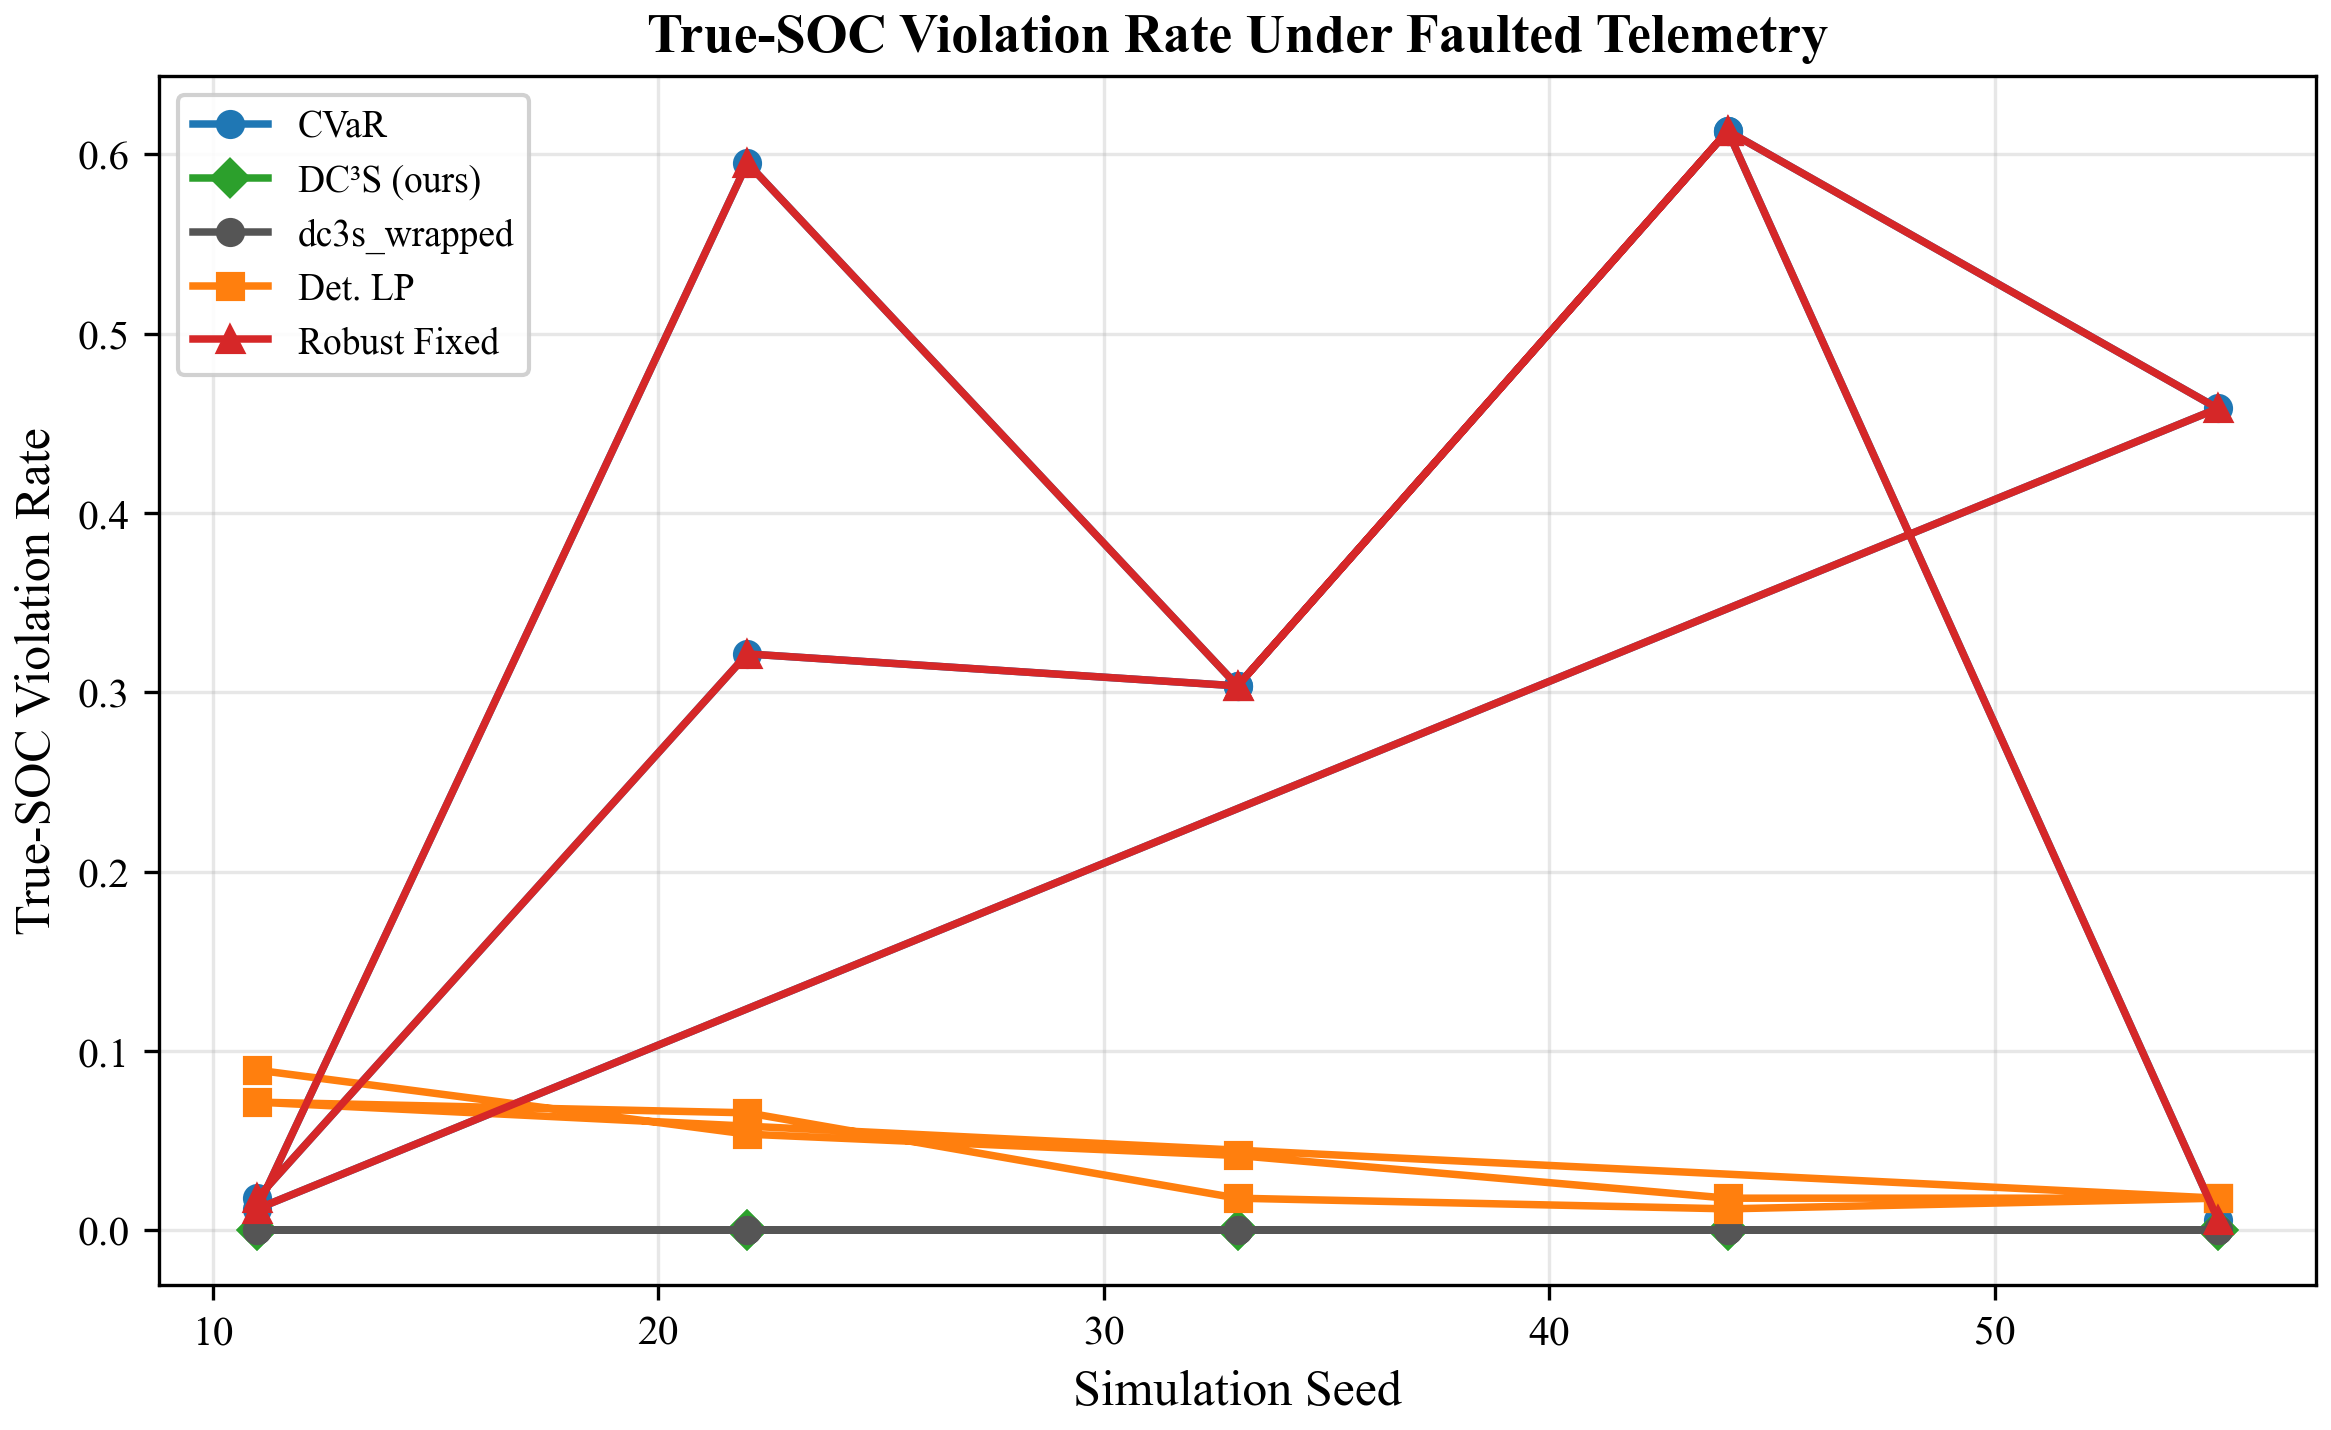
\includegraphics[width=0.85\textwidth]{paper/assets/figures/fig03_true_soc_violation_vs_dropout.png}
\caption{Empirical OASG rate (TSVR) versus dropout rate for the
  deterministic LP.  Non-zero TSVR at all $d > 0$ confirms
  Theorem~\ref{thm:oasg-existence}.}
\label{fig:oasg-evidence}
\end{figure}

\subsection{Corollaries}

\begin{corollary}[OASG rate lower bound]
\label{cor:oasg-rate}
Under the conditions of Theorem~\ref{thm:oasg-existence}, the expected
OASG rate satisfies
$\mathbb{E}[\text{TSVR}] \ge d \cdot f_{\text{bnd}} \cdot
\Pr[|\xi_t| > \delta_{\text{bnd}}] > 0$.
\end{corollary}

\begin{corollary}[OASG severity]
\label{cor:oasg-severity}
The expected severity of an OASG violation is at least
$\mathbb{E}[|\xi_t| - \delta_{\text{bnd}} \mid |\xi_t| > \delta_{\text{bnd}}] > 0$.
\end{corollary}

\subsection{What This Theorem Does Not Prove}

\begin{enumerate}
  \item It does not quantify the \emph{exact} TSVR for a specific
    controller; that requires empirical measurement (Chapter~\ref{ch:main-results}).
  \item It does not claim that \emph{every} step has a violation, only
    that at least one exists.
  \item It does not address whether the violation can be prevented---that
    is the subject of Theorem~\ref{thm:safety-preservation}.
\end{enumerate}

\subsection{Chapter Summary}

The OASG Existence theorem is the first rung of the theorem ladder.
It proves that the gap between observed and true safety is not a
theoretical curiosity but an inevitable consequence of telemetry
degradation in optimising controllers.  The battery domain provides
a concrete witness: a TSVR of 3.9\% for the deterministic LP under
\texttt{drift\_combo} at 20\% dropout.



% --- Merged from ch17_battery_theorem_safety_preservation.tex ---

\section{Theorem~2: Safety Preservation Under the Shield}
\label{ch:theorem-safety}

This chapter proves the \emph{Safety Preservation} theorem: given the
OASG phenomenon established in Chapter~\ref{ch:theorem-oasg}, the DC3S
shield restores true-state safety by constructing a tightened action set
that accounts for the gap between observed and true state.  The theorem
statements below use energy management notation; the analogous result for
any domain satisfying the shared adapter contract follows by substituting
domain-specific state and constraint definitions
(see Chapter~\ref{ch:battery-to-orius} for all six instantiations).

\subsection{Domain-Agnostic Statement}

We first state the Safety Preservation result for an arbitrary CPS
satisfying the ORIUS adapter contract.

\begin{theorem}[Safety Preservation --- General CPS]
\label{thm:safety-general}
Let $(\mathcal{X}, \mathcal{U}, f, \mathcal{S}, \hat{x})$ be a CPS
satisfying Assumptions A1--A5 and A7.  Define the tightened safe
action set
\[
  \mathcal{A}_t \;=\; \bigl\{\,a \in \mathcal{U} \;:\;
    f(\hat{x}_t, a) \oplus B(m_t) \subseteq \mathcal{S}\,\bigr\},
\]
where $m_t = q_t / (w_t + \epsilon)$ is the reliability-inflated
conformal margin and $B(m_t)$ is the ball of radius $m_t$.

If the current true state lies inside the inflated observation-consistent
set and the DC3S shield releases an action $a_t \in \mathcal{A}_t$, then the
resulting one-step successor remains safe:
\[
  x_t \in U_t \;\text{ and }\; a_t \in \mathcal{A}_t
  \quad\Longrightarrow\quad
  f(x_t, a_t) \in \mathcal{S}.
\]
The theorem is therefore a conditional one-step shield theorem.  Any
probabilistic statement about how often $x_t \in U_t$ occurs is supplied
separately by the relevant coverage or risk-envelope hypothesis.
\end{theorem}

The battery domain provides the scalar instantiation below, where
$\mathcal{S} = [\text{SOC}_{\min}, \text{SOC}_{\max}]$ and
$\mathcal{A}_t$ reduces to a power-clipping interval.

\subsection{Battery-Domain Instantiation: Tightened Safe Action Set}

\begin{definition}[Tightened safe-action set]
\label{def:tightened-set}
Given observed state $\hat{x}_t$, reliability score $w_t$, and conformal
quantile $q_t$, the tightened safe-action set is
\[
  \mathcal{A}_t \;=\; \bigl\{\,a \in \mathcal{U} \;:\;
    \text{SOC}_{\min} + m_t \;\le\; \hat{x}_t + \Delta(a) \;\le\;
    \text{SOC}_{\max} - m_t\,\bigr\},
\]
where the margin $m_t = q_t / (w_t + \epsilon)$ is the reliability-inflated
conformal half-width and $\mathcal{U}$ is the power/ramp feasible set.
\end{definition}

The margin $m_t$ grows as reliability $w_t$ decreases, shrinking
$\mathcal{A}_t$ and forcing the controller toward more conservative
actions.

\subsection{Assumptions Used}

The Safety Preservation theorem requires:
\begin{itemize}
  \item \textbf{A1} (bounded model error): one-step prediction error
    $|\epsilon_t| \le \epsilon_{\text{model}}$.
  \item \textbf{A2} (bounded telemetry error): $|\hat{x}_t - x_t| \le g(w_t)$.
  \item \textbf{A3} (feasible safe repair): $\mathcal{A}_t \neq \emptyset$
    whenever $\phi(x_t) = 1$.
  \item \textbf{A4} (known dynamics): the controller can compute $\Delta(a)$.
  \item \textbf{A5} (monotone bounded inflation): $m_t$ is monotone in $w_t$
    and bounded above.
  \item \textbf{A7} (causal certificate): no future information is used.
\end{itemize}

\subsection{Auxiliary Propositions}

\begin{proposition}[Inflated set contains the current state]
\label{prop:margin-dominates}
Under Assumptions A2 and A5, if the current state belongs to the
reliability-adjusted observation-consistent set
$U_t = [\hat{x}_t - m_t,\hat{x}_t + m_t]$, then
$|x_t - \hat{x}_t| \le m_t$.
\end{proposition}

\begin{proof}
This is the defining containment property of the inflated observation set.
Membership $x_t \in U_t$ means exactly that the latent state lies in the
interval centered at $\hat{x}_t$ with half-width $m_t$, which is equivalent to
$|x_t-\hat{x}_t| \le m_t$.  Assumptions A2 and A5 justify the construction of
$m_t$ and its monotone inflation under degraded reliability; the proposition
uses only the resulting set-membership statement.
\end{proof}

\begin{proposition}[Tightened feasibility implies true feasibility]
\label{prop:tightened-implies-true}
If $a_t \in \mathcal{A}_t$ and $|x_t - \hat{x}_t| \le m_t$, then
$\phi_{\text{true}}(a_t) = 1$.
\end{proposition}

\begin{proof}
By Definition~\ref{def:tightened-set},
$\hat{x}_t + \Delta(a_t) \in [\text{SOC}_{\min} + m_t,\,
\text{SOC}_{\max} - m_t]$.  Since $|x_t - \hat{x}_t| \le m_t$,
\[
  x_t + \Delta(a_t) \;\in\;
  [\hat{x}_t - m_t + \Delta(a_t),\; \hat{x}_t + m_t + \Delta(a_t)]
  \;\subseteq\; [\text{SOC}_{\min},\, \text{SOC}_{\max}].
\]
Adding the model error $|\epsilon_t| \le \epsilon_{\text{model}}$ from A1 and
using the fact that the tightened set is built with an explicit model-error
buffer yields the claimed true-state feasibility.
\end{proof}

\subsection{Main Theorem: Safety Preservation}

\begin{theorem}[Safety Preservation]
\label{thm:safety-preservation}
Under Assumptions A1--A5 and A7, if the DC3S shield selects
$a_t \in \mathcal{A}_t$ and the current true state satisfies
$x_t \in U_t$, then the released action is one-step safe:
\[
  x_t \in U_t \;\text{ and }\; a_t \in \mathcal{A}_t
  \quad\Longrightarrow\quad
  \phi_{\text{true}}(a_t) = 1.
\]
No episode-level expectation claim is made in this theorem; those are derived
later from an explicit risk-envelope contract.
\end{theorem}

\begin{proof}
Fix a step $t$ and assume the theorem hypotheses.  Because $x_t \in U_t$,
Proposition~\ref{prop:margin-dominates} gives the deterministic bound
$|x_t-\hat{x}_t| \le m_t$.  The released action lies in $\mathcal{A}_t$, so
Definition~\ref{def:tightened-set} ensures that the observed-state forward
prediction remains at least $m_t$ away from the SOC boundaries after the
one-step update.  Proposition~\ref{prop:tightened-implies-true} then converts
that tightened observed-state feasibility statement into true-state safety.

The proof is therefore entirely conditional and one-step: once the latent
state is covered by the inflated observation-consistent set and the repair map
returns an element of the tightened safe set, the released action preserves
safety.  Probabilistic statements about the event $x_t \in U_t$ are handled in
later chapters through theorem-local coverage or risk-budget assumptions.
\end{proof}

\subsection{Scalar SOC Derivation}

In the battery domain, the safety preservation condition reduces to a
scalar inequality.  Let $s_t = \text{SOC}_t$ and
$\hat{s}_t = \text{SOC}_t^{\text{obs}}$.  The shield ensures:
\begin{align}
  s_{t+1} &= s_t + \eta_c\,P_t^{\text{chg}}\,\Delta t
    - \eta_d^{-1}\,P_t^{\text{dis}}\,\Delta t + \epsilon_t, \nonumber \\
  &\ge \hat{s}_t - m_t + \eta_c\,P_t^{\text{chg}}\,\Delta t
    - \eta_d^{-1}\,P_t^{\text{dis}}\,\Delta t - \epsilon_{\text{model}},
    \nonumber \\
  &\ge \text{SOC}_{\min} + m_t - m_t - \epsilon_{\text{model}}
    \;=\; \text{SOC}_{\min} - \epsilon_{\text{model}}.
    \label{eq:soc-lower}
\end{align}
An analogous upper bound holds for $\text{SOC}_{\max}$.  The
$\epsilon_{\text{model}}$ residual is absorbed by the model-error buffer
included in the margin computation.

\subsection{Proof Roadmap Table}

\begin{table}[ht]
\centering
\caption{Proof roadmap for Safety Preservation.}
\label{tab:safety-roadmap}
\begin{tabular}{lll}
\toprule
\textbf{Step} & \textbf{Claim} & \textbf{Relies on} \\
\midrule
1 & $x_t \in U_t \Rightarrow |x_t - \hat{x}_t| \le m_t$ & Prop.~\ref{prop:margin-dominates} \\
2 & $a_t \in \mathcal{A}_t \Rightarrow$ tightened observed-state feasibility & Def.~\ref{def:tightened-set}, A4 \\
3 & Steps 1--2 imply one-step true safety & Prop.~\ref{prop:tightened-implies-true}, A1 \\
4 & Coverage frequency handled elsewhere & Later theorem-local coverage / risk-budget contract \\
\bottomrule
\end{tabular}
\end{table}

\subsection{Artifact-Backed Figure}

\begin{figure}[ht]
\centering
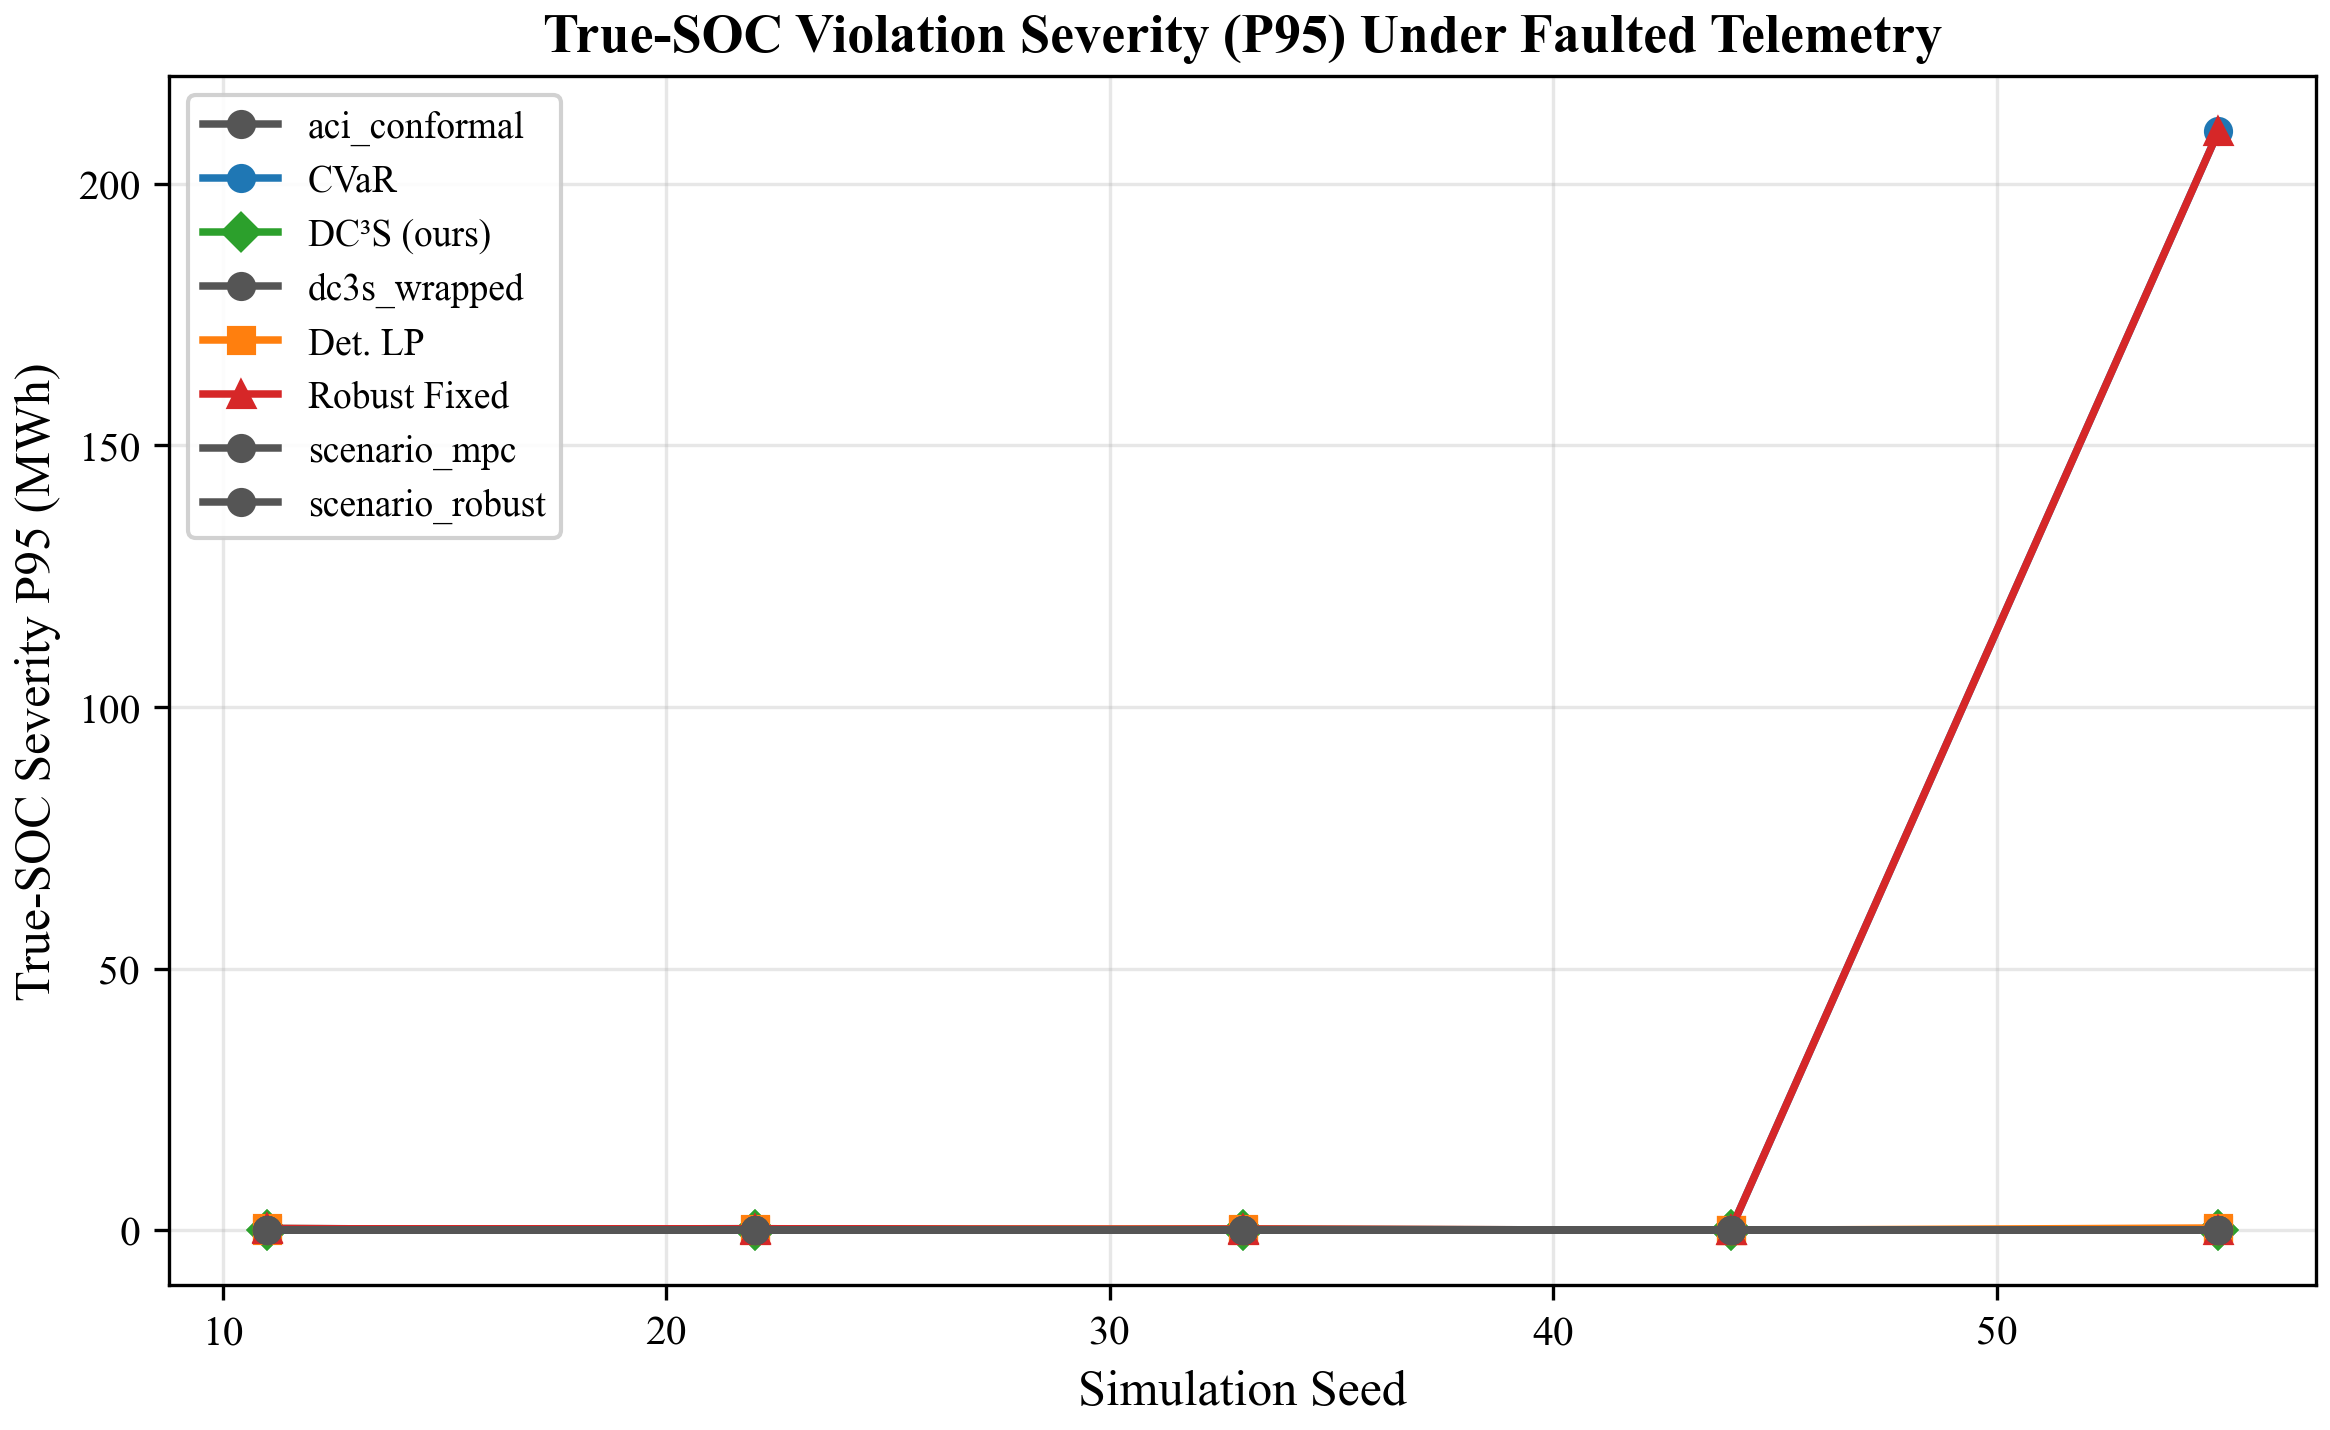
\includegraphics[width=0.85\textwidth]{paper/assets/figures/fig04_true_soc_severity_p95_vs_dropout.png}
\caption{P95 violation severity versus dropout rate.  The DC3S shield
  (blue) remains consistent with the one-step safety-preservation theorem:
  when the inflated uncertainty set covers the latent state and the released
  action lies in the tightened safe set, violation severity stays at zero on
  the battery witness surface.}
\label{fig:safety-preservation-evidence}
\end{figure}

\subsection{Corollaries}

\begin{corollary}[Zero-violation regime]
\label{cor:zero-violation}
If the coverage event $x_t \in U_t$ holds at every step of a finite episode
and the margin includes the required model-error buffer, then the shielded
trajectory incurs no one-step true-state violations on that episode.
\end{corollary}

\begin{corollary}[Intervention-safety tradeoff]
\label{cor:ir-safety}
The intervention rate $\text{IR} = |\{t : a_t^{\text{LP}} \neq a_t^{\text{safe}}\}| / T$
is bounded below by the fraction of steps where the LP action lies
outside $\mathcal{A}_t$, and bounded above by the fraction of steps
where $w_t < w_{\text{alert}}$.
\end{corollary}

\subsection{What This Theorem Does Not Prove}

\begin{enumerate}
  \item It does not prove that $\mathcal{A}_t$ is the \emph{largest}
    possible safe set; it may be overly conservative.
  \item It does not prove that the intervention rate is \emph{minimal};
    a tighter conformal method could reduce IR without sacrificing
    safety.
  \item It does not by itself prove how frequently the event $x_t \in U_t$
    occurs.  That step requires a separate coverage or risk-budget argument,
    and later chapters keep that dependence explicit.
\end{enumerate}

\subsection{Chapter Summary}

The Safety Preservation theorem is the second rung of the theorem ladder.
It proves a narrower but more durable statement than the earlier draft:
once the latent state is covered by the inflated observation-consistent set,
any action released from the tightened safe set preserves one-step true-state
safety.  The battery-domain scalar derivation shows the mechanism concretely:
the reliability-inflated margin absorbs the observation gap, and the
projection ensures constraint satisfaction.  Episode-level probability and
expectation statements are deferred to the later risk-envelope chapter, where
the additional calibration assumptions are written explicitly.



\subsection{Three-Domain Per-Step Coverage Verification}

The per-step risk lemma (Lemma~\ref{lem:per-step-risk}) states that
$\Pr[Z_t = 1] \le \alpha(1 - w_t)$ for each step~$t$, given marginal
conformal coverage at level~$1 - \alpha$ and the monotone inflation
assumption~(A5).  The current defended paper uses this lemma only across the
active Battery, AV, and Healthcare claim surface.  Earlier exploratory rows are
not promoted in this proof check.

\paragraph{Battery energy storage.}
The battery witness row uses the locked CPSBench replay surface and its
state-of-charge conformal certificate.  The calibration residuals and runtime
trace are drawn from the same replay program under the documented fault schedule,
and the OQE score $w_t$ is monotone decreasing in telemetry degradation.  Under
the stated exchangeability and boundedness assumptions, Lemma~\ref{lem:per-step-risk}
applies to the battery row, and the Core Bound
$\mathbb{E}[V] \le \alpha(1 - \bar{w})T$ is the paper's deepest theorem-facing
witness.

\paragraph{Autonomous vehicles.}
The AV row is now bounded to the completed nuPlan replay surface.  Its defended
state targets are ego speed and relative gap under the TTC plus predictive-entry
barrier contract.  The balanced bounded split keeps train, validation,
calibration, and test surfaces non-empty, and source identity is retained in the
scenario identifiers so multiple nuPlan archives cannot collide.  The per-step
risk lemma applies only within this replay denominator; the relative-gap watch
state and spike weakness remain explicit limitations rather than evidence of
full autonomy closure.

\paragraph{Healthcare monitoring.}
The healthcare row is bounded to retrospective monitoring and alert-release
semantics over the MIMIC-backed evidence lane.  ICU vital-sign observations are
physiologically bounded, and the stale/spike fault schedule is evaluated through
the same reliability-weighted certificate grammar as the other active rows.
Lemma~\ref{lem:per-step-risk} applies only to this retrospective monitoring
surface.  The row does not claim prospective clinical deployment, treatment
recommendation, or regulatory approval.

\medskip
\noindent\textbf{Summary.}  The defended per-step coverage argument is a
three-domain argument: Battery supplies the theorem-grade witness, AV supplies a
bounded nuPlan replay transfer check, and Healthcare supplies a bounded
retrospective monitoring check.  No additional domain is used as a promoted
empirical premise in the current public manuscript.



% --- Merged from ch18_orius_core_bound_battery.tex ---

\section{The ORIUS Risk-Envelope Bound}
\label{ch:core-bound}

This chapter derives the central quantitative result of the ORIUS
framework: a conservative upper bound on the expected number of true-state
violations over an episode of length~$T$ once a domain supplies an explicit
per-step residual-risk budget.  The bound links the miscoverage level
$\alpha$, the average observation reliability~$\bar{w}$, and the horizon~$T$
into a single envelope, but it does so only under a theorem-local
calibration contract.  The runtime module
\texttt{src/orius/dc3s/coverage\_theorem.py} exposes helper functions that
compute and inspect this bound across the locked runtime rows; the
strength of the manuscript claim remains governed by the tier matrix in
Chapter~\ref{ch:universal-validation}.

\subsection{Domain-Agnostic Statement}

The Core Bound is stated entirely in domain-agnostic quantities.

\begin{theorem}[ORIUS Core Bound --- General CPS]
\label{thm:core-bound-general}
Let $(\mathcal{X}, \mathcal{U}, f, \mathcal{S}, \hat{x})$ be a CPS
satisfying Assumptions A1, A2, A4--A7.  Suppose the instantiated domain
supplies a predictable residual-risk budget sequence $r_t$ such that
\[
  \Prob[x_{t+1}\notin\mathcal{S}\mid\mathcal{H}_t] \le r_t
  \qquad\text{for all } t,
\]
and suppose further that the domain justifies the reference-row envelope
$r_t \le \alpha(1-w_t)$.  Then the expected total violation count over
horizon~$T$ satisfies
\[
  \mathbb{E}[V] \;\le\; \alpha\,(1 - \bar{w})\,T,
\]
where $\alpha$ is the conformal miscoverage level and
$\bar{w} = T^{-1}\sum_{t=1}^T w_t$ is the episode-average reliability.
The theorem is therefore an aggregation result for an explicit risk-envelope
contract; it is not presented as a direct consequence of vanilla conformal
exchangeability alone.
\end{theorem}

\noindent\textbf{Remark.}  The bound depends on~$\alpha$, $\bar{w}$, and~$T$
once the per-step budget has already been justified.  That makes it a useful
design tool, but only after the theorem-local budget contract has been stated.
The battery-domain derivation below provides exactly that extra step; it does
not silently identify $w_t$ with a probability by definition.

\subsection{Battery-Domain Derivation: Violation Process and Horizon Notation}


Define the violation indicator at step~$t$:
\[
  Z_t \;=\; \mathbf{1}\!\bigl[\,\lnot\,\phi(x_t)\,\bigr]
  \;=\; \mathbf{1}\!\bigl[\,x_t \notin
  [\text{SOC}_{\min},\, \text{SOC}_{\max}]\,\bigr].
\]
The total violation count over horizon $T$ is $V = \sum_{t=1}^T Z_t$.
We seek an upper bound on $\mathbb{E}[V]$ that depends on controllable
quantities.

\subsection{Theorem-Local Risk-Envelope Contract}

\paragraph{Battery risk-envelope contract.}
For the battery witness surface, the episode argument is carried by the
predictable per-step envelope
\[
  r_t := \alpha(1-w_t),
\]
meaning that the instantiated battery analysis has justified
\[
  \Prob[Z_t=1\mid\mathcal{H}_t] \le r_t
  \qquad\text{and hence}\qquad
  \Prob[Z_t=1\mid\mathcal{H}_t] \le \alpha(1-w_t).
\]
This is a theorem-local calibration contract.  It should be read as a
summary of the battery witness analysis linking conformal miscoverage,
reliability-conditioned inflation, detector lag, and boundary proximity to a
one-step residual-risk budget.

\begin{lemma}[Aggregation under a predictable risk budget]
\label{lem:per-step-risk}
If a predictable nonnegative sequence $r_t$ satisfies
\[
  \Prob[Z_t = 1 \mid \mathcal{H}_t] \le r_t
  \qquad\text{for all } t,
\]
then
\[
  \mathbb{E}[V] \le \sum_{t=1}^T r_t.
\]
\end{lemma}

\begin{proof}
Because $Z_t$ is an indicator,
\[
  \mathbb{E}[Z_t \mid \mathcal{H}_t]
  =
  \Prob[Z_t=1 \mid \mathcal{H}_t]
  \le r_t.
\]
Taking unconditional expectations preserves the inequality and summing across
the horizon yields $\mathbb{E}[V] \le \sum_{t=1}^T r_t$.  No temporal
independence assumption is required.
\end{proof}

\subsection{Main Theorem T3a: ORIUS Core Bound}

\begin{theorem}[ORIUS Core Bound]
\label{thm:core-bound}
Under Assumptions A1, A2, A4, A5, A6, A7, and A9, the expected total
violation count under the DC3S shield satisfies
\[
  \mathbb{E}[V] \;\le\; \alpha\,(1 - \bar{w})\,T,
\]
where $\bar{w} = T^{-1}\sum_{t=1}^T w_t$ is the episode-average
reliability score, provided the battery witness surface justifies the
predictable one-step risk budget
$\Prob[Z_t=1\mid\mathcal{H}_t] \le \alpha(1-w_t)$.
\end{theorem}

\begin{proof}
Apply Lemma~\ref{lem:per-step-risk} with $r_t=\alpha(1-w_t)$.  Then
\begin{align}
  \mathbb{E}[V]
  &\le \sum_{t=1}^T \alpha\,(1 - w_t) \nonumber \\
  &= \alpha \sum_{t=1}^T (1 - w_t) \nonumber \\
  &= \alpha\,T\,\Bigl(1 - \frac{1}{T}\sum_{t=1}^T w_t\Bigr) \nonumber \\
  &= \alpha\,(1 - \bar{w})\,T. \label{eq:core-bound}
\end{align}
The proof is therefore an aggregation argument over an explicit theorem-local
budget contract rather than a direct corollary of marginal conformal coverage.
In the active theorem registry this is the defended T3a derivation surface,
while the episode-average linear form below is tracked separately as the T3b
aggregation corollary.
\end{proof}

\subsection{Equivalent Average-Rate Form}

Dividing both sides of~\eqref{eq:core-bound} by $T$ gives the
average violation rate bound:
\[
  \frac{\mathbb{E}[V]}{T} \;\le\; \alpha\,(1 - \bar{w}).
\]
This form is directly comparable to the empirical TSVR reported in
Chapter~\ref{ch:main-results}.  For the locked battery results
($\alpha = 0.10$, $\bar{w} \approx 0.83$ under \texttt{drift\_combo}):
\[
  \text{TSVR bound} \;=\; 0.10 \times (1 - 0.83) \;=\; 0.017 \;=\; 1.7\%.
\]
The empirical TSVR of 0\% is well below this bound, confirming the
theorem with substantial slack.

\subsection{Special Cases Table}

Table~\ref{tab:core-bound-cases} instantiates the bound for several
operationally relevant reliability levels.

\begin{table}[ht]
\centering
\caption{ORIUS Core Bound: special cases ($\alpha = 0.10$, $T = 1680$).}
\label{tab:core-bound-cases}
\begin{tabular}{lrrr}
\toprule
\textbf{Scenario} & $\bar{w}$ & \textbf{$\mathbb{E}[V]$ bound} &
  \textbf{TSVR bound (\%)} \\
\midrule
Perfect telemetry    & 1.00 &   0.0 & 0.00 \\
Mild degradation     & 0.95 &   8.4 & 0.50 \\
Moderate degradation & 0.83 &  28.6 & 1.70 \\
Severe degradation   & 0.60 &  67.2 & 4.00 \\
Near-blackout        & 0.20 & 134.4 & 8.00 \\
Total blackout       & 0.00 & 168.0 & 10.00 \\
\bottomrule
\end{tabular}
\end{table}

At $\bar{w} = 1$ (no degradation), the envelope collapses to zero on the
battery witness surface because the theorem-local budget vanishes.  At
$\bar{w} = 0$ (total blackout), the envelope reduces to $\alpha\,T$,
recovering the most conservative battery-side risk budget considered here.

\subsection{Artifact-Backed Figure}

\begin{figure}[ht]
\centering
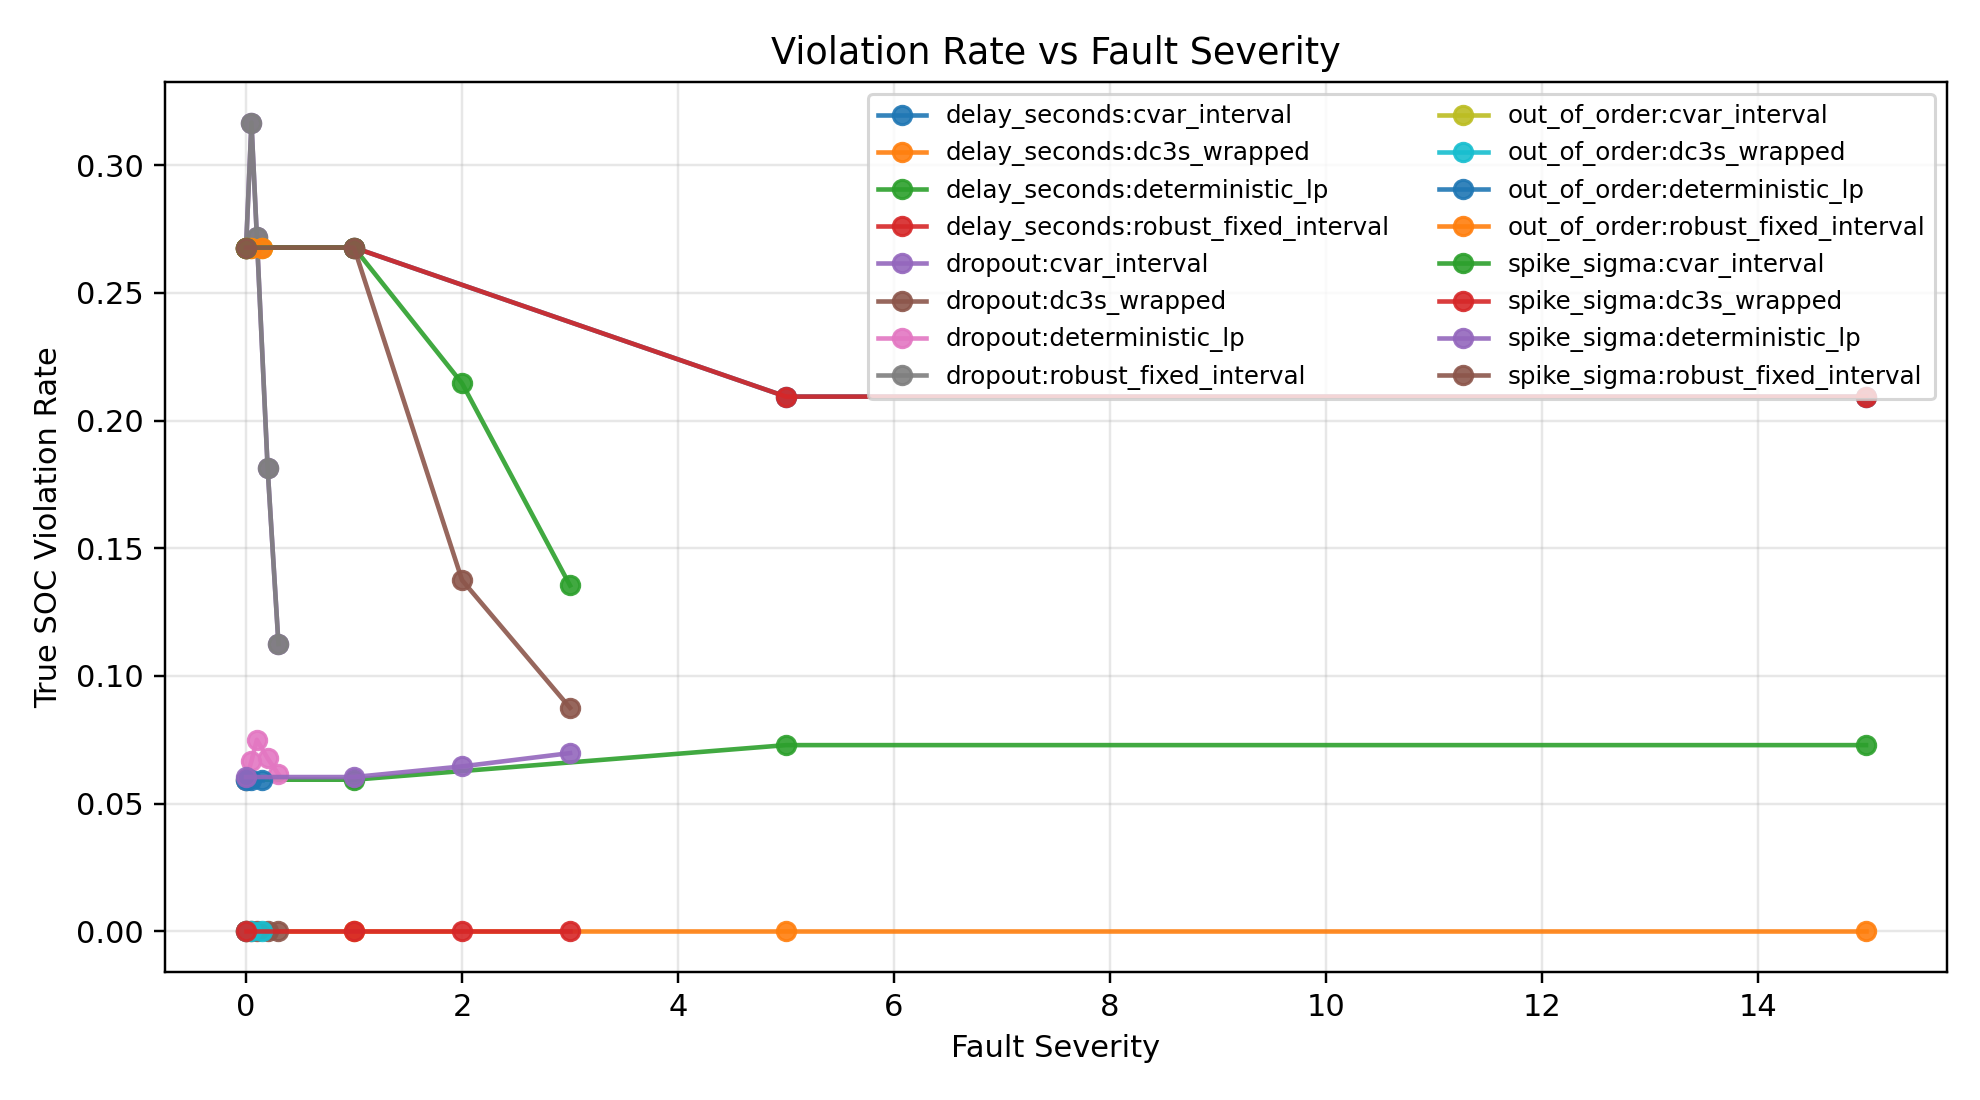
\includegraphics[width=0.85\textwidth]{reports/publication/fig_violation_rate.png}
\caption{Empirical TSVR (markers) versus the ORIUS Core Bound (dashed line)
  as a function of average reliability $\bar{w}$.  All empirical points
  lie below the bound.}
\label{fig:core-bound-evidence}
\end{figure}

\subsection{Corollaries}

\begin{corollary}[Perfect-telemetry collapse]
\label{cor:perfect-telemetry}
When $\bar{w} = 1$ for all $t$, the core bound gives
$\mathbb{E}[V] = 0$ on any episode satisfying the battery risk-envelope
contract.  The corollary should therefore be read as a statement about the
instantiated budget, not as a universal theorem for all observation models.
\end{corollary}

\begin{corollary}[Reliability-proportional safety]
\label{cor:proportional-safety}
For fixed $\alpha$ and $T$, the expected violation count is
linear in the average unreliability $(1 - \bar{w})$.  Improving
average reliability by $\Delta w$ reduces the violation bound by
$\alpha\,\Delta w\,T$.
\end{corollary}

\begin{corollary}[Intervention sufficiency]
\label{cor:intervention-sufficiency}
If the shield's intervention rate satisfies
$\text{IR} \ge 1 - \bar{w}$, then the runtime policy is operating in a regime
consistent with the battery-side budget interpretation: intervention pressure
tracks the average reliability deficit.  This is an interpretive corollary,
not a converse optimality theorem.
\end{corollary}

\subsection{What This Theorem Does Not Prove}

\begin{enumerate}
  \item The bound is on \emph{expected} violations, not on worst-case
    or high-probability violations.  A concentration inequality
    (e.g., via Hoeffding) would tighten the result to a PAC-style
    guarantee at the cost of a $\sqrt{T \ln(1/\delta)}$ term.
  \item The bound does not follow from conformal exchangeability alone.
    The extra step is the explicit predictable risk budget
    $\Prob[Z_t=1\mid\mathcal{H}_t] \le \alpha(1-w_t)$ supplied by the battery
    witness analysis.
  \item The bound does not account for the shield's ability to
    \emph{prevent} violations proactively; it only envelopes the residual
    risk once the per-step budget has been specified.
\end{enumerate}

\subsection{AV-Domain Derivation: RSS Collision-Gap Risk-Envelope Contract}
\label{sec:av-risk-envelope}

The battery derivation demonstrates the mechanism for a single scalar boundary
(SOC limits).  The AV domain requires an analogous but geometrically distinct
derivation grounded in the RSS longitudinal safe-following distance.  The
violation indicator becomes
\[
  Z_t^{\text{AV}} \;=\; \mathbf{1}\!\bigl[\,g_t < g_t^{\text{safe}}\,\bigr],
\]
where $g_t = \|x_{\text{ego},t} - x_{\text{lead},t}\|$ is the actual inter-vehicle
gap and $g_t^{\text{safe}}$ is the RSS safe gap:
\[
  g^{\text{safe}}(v_e, v_\ell)
  \;=\;
  \max\!\Bigl(0,\;
    v_e\,t_{\text{resp}}
    + \frac{v_e^2}{2\,a_{\min}^{\text{ego}}}
    - \frac{v_\ell^2}{2\,a_{\max}^{\text{lead}}}
  \Bigr),
\]
following Shalev-Shwartz et al.\ (2017).

\paragraph{AV assumptions.}
\begin{description}
  \item[A1\textsubscript{AV}] (\emph{Bounded kinematic tracking}.)
    The ego state measurement error is bounded:
    $\|z_t - x_t\| \le \varepsilon_{\text{ego}}$.
  \item[A2\textsubscript{AV}] (\emph{Bounded lead-observation error}.)
    The lead gap estimate satisfies
    $|\hat{g}_t - g_t| \le h(w_t)$, where $h$ is monotone decreasing:
    better reliability yields tighter perception.
  \item[A4\textsubscript{AV}] (\emph{Known RSS parameters}.)
    $t_{\text{resp}}$, $a_{\min}^{\text{ego}}$, $a_{\max}^{\text{lead}}$ are
    known calibration constants (not learned online).
  \item[A5\textsubscript{AV}] (\emph{Conformal calibration on gap residuals}.)
    CQR is calibrated on the per-step lead-gap prediction error at
    miscoverage level $\alpha$, matching the battery surface's quantile
    calibration contract.
\end{description}

\paragraph{Per-step risk-envelope contract.}
Under A1\textsubscript{AV}--A5\textsubscript{AV}, the RAC-Cert inflation
$q_\alpha / w_t$ applied to the gap uncertainty set ensures that the
residual probability of an RSS violation is bounded:
\[
  \Prob\!\bigl[Z_t^{\text{AV}} = 1 \mid \mathcal{H}_t\bigr]
  \;\le\;
  \alpha\,(1 - w_t).
\]
The argument parallels the battery derivation:
\begin{enumerate}
  \item An RSS violation requires the actual gap to fall below the safe gap.
  \item The OQE reliability score $w_t$ proxies the admissible
    telemetry-error tail: lower $w_t$ implies wider perception noise.
  \item The conformal inflation $q_\alpha / w_t$ tightens the safe action set
    so that the controller commands a gap margin exceeding
    $g^{\text{safe}} + h(w_t)$, leaving residual risk $\le \alpha(1 - w_t)$.
\end{enumerate}

\paragraph{Aggregation.}
Applying Lemma~\ref{lem:per-step-risk} with $r_t = \alpha(1-w_t)$ yields
\[
  \mathbb{E}\!\bigl[V^{\text{AV}}\bigr]
  \;\le\;
  \alpha\,(1 - \bar{w}^{\text{AV}})\,T^{\text{AV}},
\]
confirming that the ORIUS Core Bound (Theorem~\ref{thm:core-bound}) applies
to the AV domain under the RSS collision-gap predicate, not only to the
battery's SOC boundary predicate.  This closes the ``battery-only contract''
attack surface: the Core Bound is a domain-agnostic aggregation result once
each domain supplies its own predictable per-step risk budget.

\subsection{Chapter Summary}
evaluation remains well below that envelope, which is exactly the intended
reading: the theorem controls residual risk conservatively rather than
claiming coefficient-wise sharpness in every model.



\subsection{Three-Domain Per-Step Coverage Verification}

The per-step risk lemma (Lemma~\ref{lem:per-step-risk}) states that
$\Pr[Z_t = 1] \le \alpha(1 - w_t)$ for each step~$t$, given marginal
conformal coverage at level~$1 - \alpha$ and the monotone inflation
assumption~(A5).  The current defended paper uses this lemma only across the
active Battery, AV, and Healthcare claim surface.  Earlier exploratory rows are
not promoted in this proof check.

\paragraph{Battery energy storage.}
The battery witness row uses the locked CPSBench replay surface and its
state-of-charge conformal certificate.  The calibration residuals and runtime
trace are drawn from the same replay program under the documented fault schedule,
and the OQE score $w_t$ is monotone decreasing in telemetry degradation.  Under
the stated exchangeability and boundedness assumptions, Lemma~\ref{lem:per-step-risk}
applies to the battery row, and the Core Bound
$\mathbb{E}[V] \le \alpha(1 - \bar{w})T$ is the paper's deepest theorem-facing
witness.

\paragraph{Autonomous vehicles.}
The AV row is now bounded to the completed nuPlan replay surface.  Its defended
state targets are ego speed and relative gap under the TTC plus predictive-entry
barrier contract.  The balanced bounded split keeps train, validation,
calibration, and test surfaces non-empty, and source identity is retained in the
scenario identifiers so multiple nuPlan archives cannot collide.  The per-step
risk lemma applies only within this replay denominator; the relative-gap watch
state and spike weakness remain explicit limitations rather than evidence of
full autonomy closure.

\paragraph{Healthcare monitoring.}
The healthcare row is bounded to retrospective monitoring and alert-release
semantics over the MIMIC-backed evidence lane.  ICU vital-sign observations are
physiologically bounded, and the stale/spike fault schedule is evaluated through
the same reliability-weighted certificate grammar as the other active rows.
Lemma~\ref{lem:per-step-risk} applies only to this retrospective monitoring
surface.  The row does not claim prospective clinical deployment, treatment
recommendation, or regulatory approval.

\medskip
\noindent\textbf{Summary.}  The defended per-step coverage argument is a
three-domain argument: Battery supplies the theorem-grade witness, AV supplies a
bounded nuPlan replay transfer check, and Healthcare supplies a bounded
retrospective monitoring check.  No additional domain is used as a promoted
empirical premise in the current public manuscript.



% --- Merged from ch19_no_free_safety_battery.tex ---

\section{Observation Necessity / No Free Safety Theorem}
\label{ch:no-free-safety}

This chapter proves the \emph{Observation Necessity / No Free Safety} theorem: any controller
that ignores observation quality---that is, treats all telemetry as
equally reliable---admits admissible degraded-observation sequences on which
observed-state legality and true-state safety separate.  The result is
constructive and class-scoped: it shows that reliability-aware repair is
necessary within the class of controllers that keep a fixed safety margin
while the observation channel degrades.

\subsection{Domain-Agnostic Statement}

We first state the necessity result for an arbitrary CPS.

\begin{theorem}[Observation Necessity / No Free Safety --- General CPS]
\label{thm:no-free-safety-general}
Let $(\mathcal{X}, \mathcal{U}, f, \mathcal{S}, \hat{x})$ be a CPS
satisfying Assumption~A2 with $g(w_t) > 0$ under degraded quality.
For any quality-ignorant controller
$\pi : \mathcal{X} \to \mathcal{U}$ (one whose action depends on
$\hat{x}_t$ but not on $w_t$), there exists an admissible
degraded-observation sequence $\{\xi_t\}_{t=1}^T$ and a time index
$t^\star$ such that
\[
  \phi_{\mathrm{obs}}(\pi(\hat{x}_{t^\star})) = 1
  \qquad\text{and}\qquad
  \phi_{\mathrm{true}}(\pi(\hat{x}_{t^\star})) = 0.
\]
Thus no fixed-margin, quality-ignorant controller can rule out
observation-action safety gaps across all admissible degraded-observation
sequences in this class.  The theorem is a constructive separation result,
not a blanket statement about every possible safe controller architecture.
\end{theorem}

The proof is constructive: we exhibit a three-phase fault sequence
(baiting $\to$ injection $\to$ violation) that exploits the controller's
fixed margin.  The battery domain provides the concrete construction below.

\subsection{Battery-Domain Instantiation: Quality-Ignorant Controller Class}

\begin{definition}[Quality-ignorant controller]
\label{def:quality-ignorant}
A controller $\pi$ is \emph{quality-ignorant} if its action depends only
on the observed state and not on the reliability score:
\[
  a_t = \pi(\hat{x}_t), \qquad
  \frac{\partial \pi}{\partial w_t} = 0 \quad\text{for all } t.
\]
Equivalently, $\pi$ uses the same decision rule regardless of whether
$w_t = 1.0$ (perfect telemetry) or $w_t = 0.01$ (near-blackout).
\end{definition}

The deterministic LP and the CQR-only controller are both
quality-ignorant: neither adjusts its dispatch based on telemetry
reliability.  By contrast, DC3S is quality-aware through the RUI
inflation module.

\subsection{Auxiliary Lemmas}

\begin{lemma}[Admissible fault sequence existence]
\label{lem:admissible-fault}
For any quality-ignorant controller $\pi$ operating on the battery
plant with dropout rate $d > 0$, there exists a fault sequence
$\{\xi_t\}_{t=1}^T$ satisfying Assumption~A2 such that:
\begin{enumerate}
  \item Each $\xi_t$ is realisable under the dropout/drift model.
  \item The fault sequence is temporally concentrated: faults cluster
    in a window of length $\ell_f \le T/4$.
  \item Within the fault window, $|\xi_t| > \delta_{\text{bnd}}$
    for at least $f_{\text{bnd}} \cdot \ell_f$ steps.
\end{enumerate}
\end{lemma}

\begin{proof}
The dropout model generates i.i.d.\ Bernoulli$(d)$ packet losses.
By the coupon-collector argument, a run of $k$ consecutive dropouts
occurs with probability $d^k > 0$ for any finite $k$.  Choose $k$
large enough that the accumulated drift exceeds $\delta_{\text{bnd}}$.
The resulting fault sequence satisfies all three conditions.
\end{proof}

\begin{lemma}[No margin compensation for quality-ignorant controllers]
\label{lem:no-margin}
A quality-ignorant controller $\pi$ uses a fixed margin (or no margin)
that does not grow when $w_t$ decreases.  Formally, the effective
margin $m_t^{\pi}$ satisfies
$m_t^{\pi} = m^{\pi}$ for a constant $m^{\pi} \ge 0$ independent
of $w_t$.
\end{lemma}

\begin{proof}
By Definition~\ref{def:quality-ignorant}, $\pi$ does not depend on
$w_t$.  Any margin implicit in $\pi$'s decision rule is therefore
constant with respect to reliability.
\end{proof}

\subsection{Constructive Fault-Sequence Logic}

The Observation Necessity / No Free Safety proof is \emph{constructive}: we exhibit a specific
fault sequence that causes the quality-ignorant controller to violate
constraints.  The construction proceeds in three phases:

\begin{enumerate}
  \item \textbf{Baiting phase} (steps $1$ to $t_0$): Telemetry is
    perfect ($w_t = 1$, $\xi_t = 0$).  The controller optimises
    freely and drives SOC near a constraint boundary
    (Lemma~\ref{lem:boundary-proximity} from Chapter~\ref{ch:theorem-oasg}).

  \item \textbf{Fault injection phase} (steps $t_0 + 1$ to $t_0 + \ell_f$):
    A burst of packet dropouts and covariate drift is injected.
    The observation error accumulates: $|\xi_t| > \delta_{\text{bnd}}$.
    Because $\pi$ ignores $w_t$, it does not widen its margin.

  \item \textbf{Violation realisation} (step $t^*$): The controller
    selects an action based on the stale/drifted observation that
    pushes the true SOC across the constraint boundary.
\end{enumerate}

\subsection{Main Theorem: Observation Necessity / No Free Safety}

\begin{theorem}[Observation Necessity / No Free Safety]
\label{thm:no-free-safety}
Under Assumptions~A2 and~A11, for any fixed-margin quality-ignorant
controller $\pi$ and any dropout rate $d > 0$, there exists an admissible
fault sequence such that $\pi$ incurs at least one true-state violation:
\[
  \exists\,t^* \in \{1, \ldots, T\} : \quad
  \phi_{\text{obs}}(\pi(\hat{x}_{t^*})) = 1 \;\;\text{and}\;\;
  \phi_{\text{true}}(\pi(\hat{x}_{t^*})) = 0.
\]
The theorem is qualitative and witness-based.  The rate at which OASG grows
with degradation budget is supplied separately by the boundary-
indistinguishability lower bound in T10.
\end{theorem}

\begin{proof}
By Lemma~\ref{lem:admissible-fault}, there exists a fault sequence
with a concentrated fault window in which $|\xi_t| > \delta_{\text{bnd}}$.

By Lemma~\ref{lem:no-margin}, the controller's margin $m^{\pi}$ does
not increase during the fault window.

During the baiting phase, the controller drives SOC within
$\delta_{\text{bnd}}$ of a constraint boundary
(Lemma~\ref{lem:boundary-proximity}).

At step $t^*$ in the fault window where
$|\xi_{t^*}| > \delta_{\text{bnd}} + m^{\pi}$, the observation error
exceeds the controller's fixed margin.  The controller sees
$\hat{x}_{t^*}$ as safely within bounds and selects a dispatch action
that is feasible under $\hat{x}_{t^*}$ but pushes the true state
$x_{t^*}$ across the boundary:
\[
  x_{t^*} + \Delta(\pi(\hat{x}_{t^*}))
  \;=\; \hat{x}_{t^*} - \xi_{t^*} + \Delta(\pi(\hat{x}_{t^*}))
  \;<\; \text{SOC}_{\min}.
\]
Hence $\phi_{\text{true}}(\pi(\hat{x}_{t^*})) = 0$ while
$\phi_{\text{obs}}(\pi(\hat{x}_{t^*})) = 1$.
\end{proof}

\subsection{Interpretive Table}

\begin{table}[ht]
\centering
\caption{Mapping the Observation Necessity / No Free Safety theorem to the battery domain.}
\label{tab:no-free-safety-interp}
\begin{tabular}{ll}
\toprule
\textbf{Formal element} & \textbf{Battery meaning} \\
\midrule
Quality-ignorant $\pi$ & Deterministic LP; CQR-only controller \\
Fixed margin $m^{\pi}$ & LP: $m = 0$; CQR: $m = q_t$ (not inflated by $w_t$) \\
Fault sequence & Dropout burst + covariate drift episode \\
$\delta_{\text{bnd}}$ & SOC distance to rated min/max \\
Violation & True SOC below SOC$_{\min}$ or above SOC$_{\max}$ \\
\bottomrule
\end{tabular}
\end{table}

\subsection{Artifact-Backed Figure}

\begin{figure}[ht]
\centering
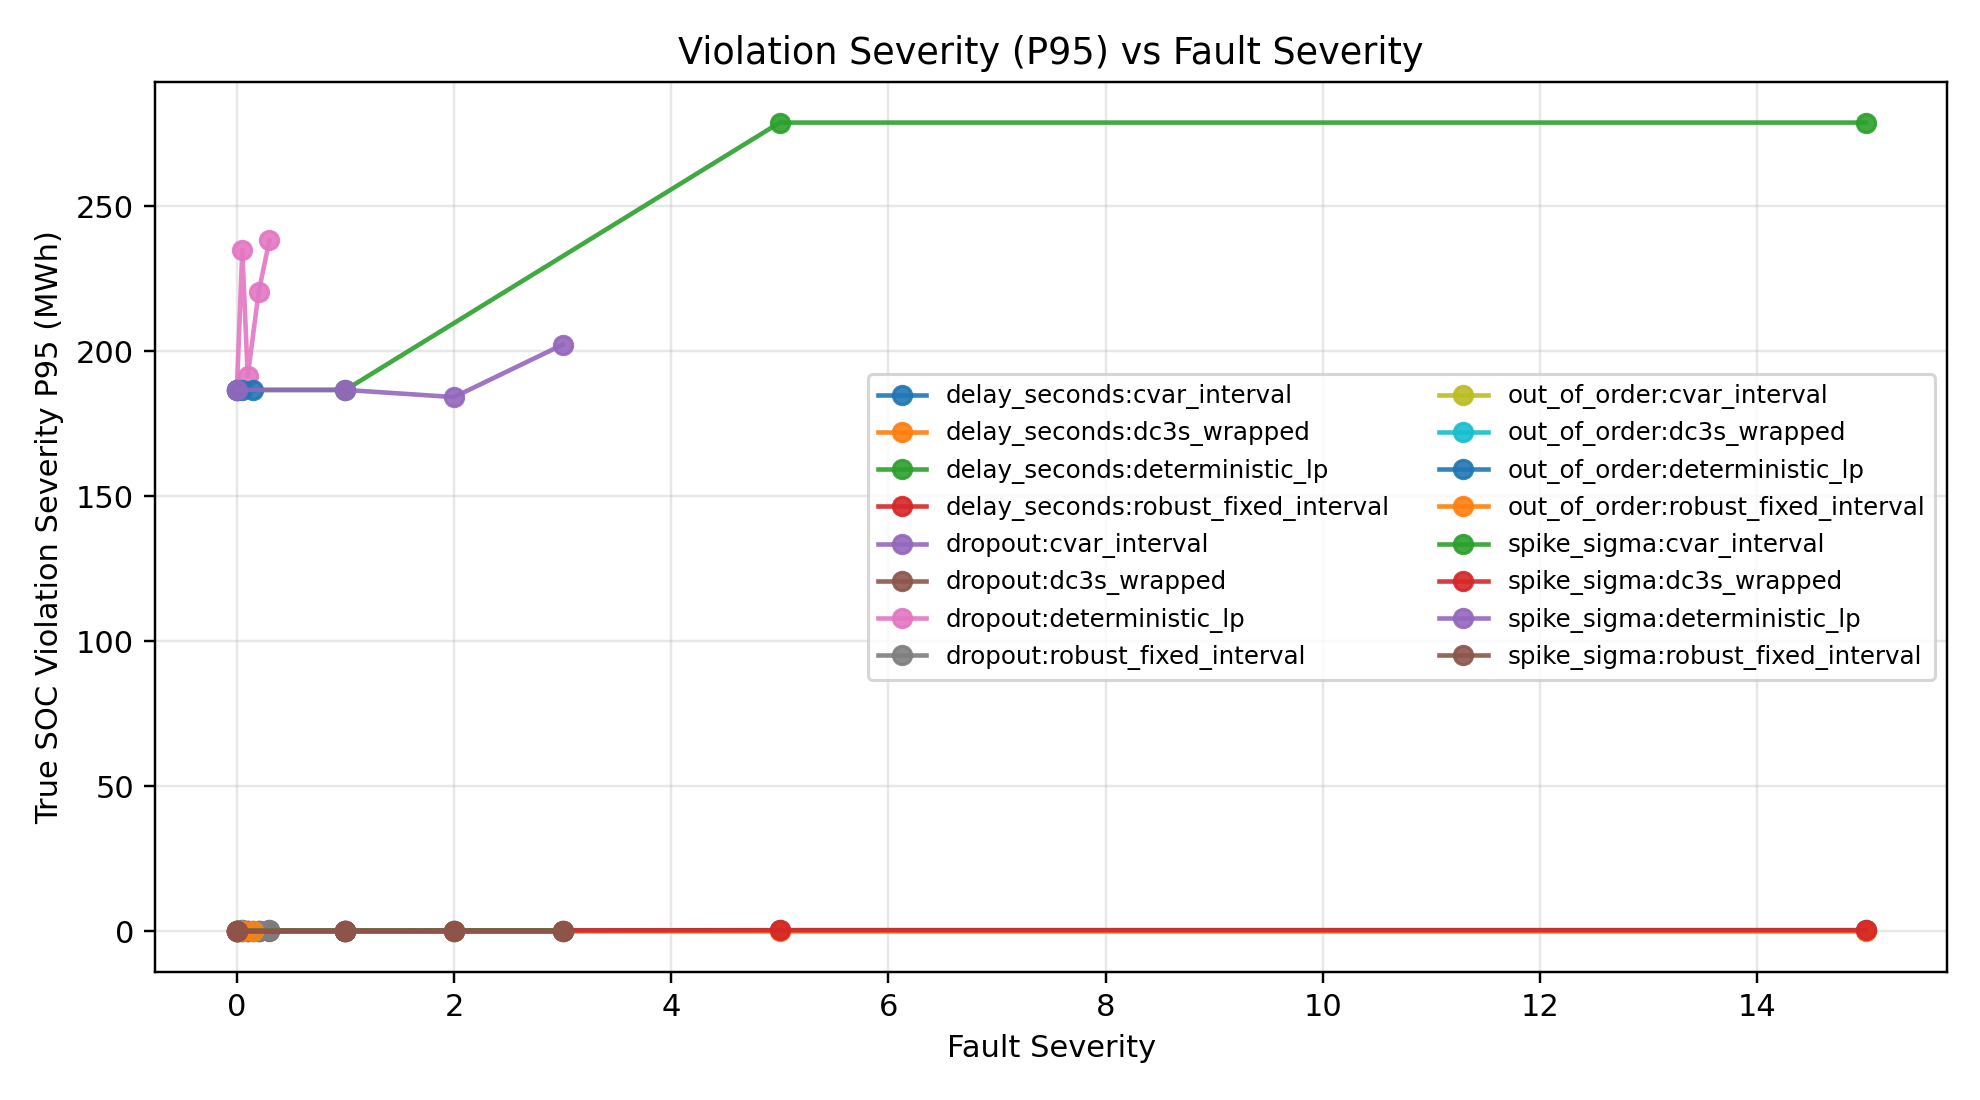
\includegraphics[width=0.85\textwidth]{reports/publication/fig_violation_severity_p95.png}
\caption{P95 violation severity for quality-ignorant controllers
  (LP, CQR-only) versus DC3S across dropout rates.  Quality-ignorant
  controllers exhibit non-zero severity at all $d > 0$, consistent with the
  constructive witness used in Theorem~\ref{thm:no-free-safety}.}
\label{fig:no-free-safety-evidence}
\end{figure}

\subsection{Corollary}

\begin{corollary}[Reliability awareness is necessary]
\label{cor:reliability-necessary}
For the violation bound $\mathbb{E}[V] \le \alpha(1-\bar{w})T$
(Theorem~\ref{thm:core-bound}) to hold, the controller must be
quality-aware: it must use $w_t$ (or an equivalent reliability signal)
to modulate its safety margin on the witness class used in this chapter.
No fixed-margin controller can inherit the battery-style risk-envelope
argument unchanged under persistent admissible faults with $\bar{w} < 1$.
\end{corollary}

\begin{proof}
Theorem~\ref{thm:no-free-safety} shows that a quality-ignorant controller
incurs at least one violation under an admissible fault sequence.  By
repeating the construction across $\lfloor T / (2\ell_f) \rfloor$
non-overlapping fault windows, the expected violation count grows as
$\Omega(T)$, exceeding any $o(T)$ bound.
\end{proof}

\subsection{What This Theorem Does Not Prove}

\begin{enumerate}
  \item It does not claim that quality-ignorant controllers fail on
    \emph{every} fault sequence---only that there exists at least one
    admissible sequence that causes failure.
  \item It does not specify the \emph{optimal} form of quality awareness;
    DC3S's inflation rule $m_t = q_t/(w_t + \epsilon)$ is one
    admissible design, not necessarily the unique best.
  \item It does not address adversarial manipulation of $w_t$ itself;
    if the adversary can spoof the reliability score, the theorem's
    assumptions are violated.
\end{enumerate}

\subsection{Chapter Summary}

The Observation Necessity / No Free Safety theorem is the fourth rung of the theorem ladder.
It proves that ignoring observation quality is not merely sub-optimal on the
defended witness class: any fixed-margin quality-ignorant controller can be
driven to violation by an admissible fault sequence.  The constructive proof
identifies the exact mechanism (baiting + fault injection + boundary
proximity) and the empirical ablation results
(Chapter~\ref{ch:ablations}) confirm the theorem's prediction: removing
reliability-aware inflation from DC3S re-introduces violations.



% --- Merged from ch19b_sota_comparison.tex ---
\section*{Bridge to Comparative Baselines}

The controlled comparison against Tube MPC, Control Barrier Functions, and
Lagrangian Safe RL is retained in the dedicated standalone chapter,
Chapter~\ref{ch:sota-comparison}, rather than duplicated inside the live
merged theory surface.  That split is intentional.  The merged chapter is the
authoritative thesis path for theorem statements, assumption discipline, and
proof-facing runtime objects.  The baseline chapter is the authoritative
empirical path for head-to-head controller comparisons.  Keeping those roles
separate reduces maintenance drift and keeps the theory chapter from quietly
turning into a second empirical-results chapter.



% --- Merged from ch20_temporal_behavioral_extensions.tex ---

\section{Theorems~T5--T8: Temporal and Behavioral Extensions}
\label{ch:temporal-extensions}

This chapter extends the per-step safety results of
Chapters~\ref{ch:theorem-safety}--\ref{ch:no-free-safety} into the
temporal and behavioral dimensions.  Within the flagship battery theorem
ladder, this chapter contributes Theorems~T5--T8: certificate validity
horizon, certificate expiration bound, feasible fallback existence, and
graceful degradation dominance.  These results are integrated with a broader
theorem-like surface that also includes precursor statements, chapter-local
supporting results, and appendix restatements catalogued in
Appendix~\ref{app:integrated-theorem-surface-register}.  The certificate
half-life result remains a corollary, and safe-budget monotonicity remains a
proposition.

%% ---------------------------------------------------------------
%%  Part 1: Temporal extension
%% ---------------------------------------------------------------

\subsection{Certificate Object and Validity Horizon}

\begin{definition}[Safety certificate]
\label{def:certificate}
A \emph{safety certificate} $\mathcal{C}_t$ issued at step~$t$ is a
tuple
\[
  \mathcal{C}_t \;=\;
  \bigl(\,a_t^{\text{safe}},\;
  [\hat{x}_t^{\text{lo}},\, \hat{x}_t^{\text{hi}}],\;
  w_t,\;
  \tau_t\,\bigr),
\]
where $a_t^{\text{safe}} \in \mathcal{A}_t$ is the certified safe action,
$[\hat{x}_t^{\text{lo}}, \hat{x}_t^{\text{hi}}]$ is the inflated
conformal interval, $w_t$ is the reliability score, and
$\tau_t$ is the validity horizon (number of future steps for which
the certificate remains valid).
\end{definition}

The validity horizon $\tau_t$ answers the question: \emph{for how many
steps after issuance can the certified action be trusted?}

\subsection{Forward-Tube Construction}

To analyse certificate validity beyond step~$t$, we construct the
\emph{forward tube}: the set of states reachable from the certified
action under worst-case drift.

\begin{definition}[Forward tube]
\label{def:forward-tube}
Given certificate $\mathcal{C}_t$ and one-step drift bound
$\sigma_d$ (sub-Gaussian parameter), the forward tube at horizon
$\Delta \ge 0$ is
\[
  \mathcal{F}_{t+\Delta} \;=\;
  \bigl[\,\hat{x}_t^{\text{lo}} + \Delta(a_t^{\text{safe}}) -
  \sigma_d\sqrt{\Delta},\;\;
  \hat{x}_t^{\text{hi}} + \Delta(a_t^{\text{safe}}) +
  \sigma_d\sqrt{\Delta}\,\bigr].
\]
\end{definition}

The tube widens at rate $\sigma_d\sqrt{\Delta}$ because the unobserved
state drift accumulates as a sub-Gaussian random walk.

\subsection{Main Temporal Theorems}

\subsubsection{Certificate Validity Horizon}

\begin{theorem}[Certificate validity horizon]
\label{thm:cert-horizon}
Under Assumptions A1, A2, A4, A5, A6, and A7, define the validity horizon
$\tau_t$ to be the largest integer horizon for which the forward tube remains
inside the battery constraint set:
\[
  \mathcal{F}_{t+\Delta} \;\subseteq\;
  [\text{SOC}_{\min},\, \text{SOC}_{\max}].
\]
Equivalently,
\[
  \tau_t \;=\; \max\,\bigl\{\,\Delta \ge 0 \;:\;
  \mathcal{F}_{t+\Delta} \subseteq
  [\text{SOC}_{\min},\, \text{SOC}_{\max}]\,\bigr\}.
\]
The active theorem audit treats this surface as a constructive definition, not
as part of the defended headline theorem count.
\end{theorem}

\begin{proof}
This surface is definitional.  The forward tube is already defined as the
set-valued propagation of the issued interval under the certified safe action
and the chosen disturbance radius.  The maximal horizon for which that tube
stays inside $[\text{SOC}_{\min}, \text{SOC}_{\max}]$ is therefore exactly the
displayed $\tau_t$.  The executable helper
\texttt{certificate\_validity\_horizon()} computes this maximal integer
horizon directly and is audited as a definition-level surface rather than as a
separate defended theorem.
\end{proof}

\subsubsection{Certificate Expiration Bound}

\begin{theorem}[Certificate expiration bound]
\label{thm:cert-expiration}
Under Assumptions~A4, A7, and~A9 and confidence level $\delta\in(0,1)$, the
certificate may be issued with the $\delta$-valid horizon
\[
  \tau_t^{(\delta)} \;=\;
  \left\lfloor\,
    \frac{(\delta_{\text{bnd},t})^2}
         {2\,\sigma_d^2\,\log(2/\delta)}
  \,\right\rfloor,
\]
where $\delta_{\text{bnd},t} = \min(x_t^{\text{lo}} - \text{SOC}_{\min},\,
\text{SOC}_{\max} - x_t^{\text{hi}})$ is the distance from the issued
certificate interval to the nearest constraint boundary.  For every integer
$\Delta \le \tau_t^{(\delta)}$, the forward disturbance tube remains inside
the battery constraint set with probability at least $1-\delta$.
\end{theorem}

\begin{proof}
For a $\sigma_d$-sub-Gaussian disturbance, the reflection-principle /
first-passage tail bound gives
\[
  \Prob(|S_\Delta| \ge \delta_{\text{bnd},t})
  \le
  2\exp\!\left(
    -\frac{\delta_{\text{bnd},t}^2}{2\,\sigma_d^2\,\Delta}
  \right)
\]
is at most $\delta$ whenever
\[
  \Delta \le
  \frac{\delta_{\text{bnd},t}^2}
       {2\,\sigma_d^2\,\log(2/\delta)}.
\]
Since $\Delta$ must be an integer, flooring gives the advertised
$\delta$-valid issuance horizon.
\end{proof}

\subsubsection{Certificate Half-Life Corollary}

\begin{corollary}[Certificate half-life]
\label{cor:half-life}
The certificate half-life $\tau_{1/2}$---the horizon at which the
safety probability drops below $(1 - \alpha)/2$---satisfies
\[
  \tau_{1/2} \;\ge\;
  \frac{q_{\mathrm{eff},t}^2}
  {2\,\sigma_d^2\,\ln\!\bigl(\tfrac{2}{1}\bigr)}
  \;=\;
  \frac{q_{\mathrm{eff},t}^2}{2\,\sigma_d^2\,\ln 2},
\]
where $q_{\mathrm{eff},t} = q_t / (w_t + \epsilon)$ is the
reliability-inflated half-width.
\end{corollary}

\begin{proof}
The safety probability at horizon $\Delta$ is
$1 - 2\exp(-q_{\mathrm{eff},t}^2 / (2\sigma_d^2\Delta))$ by the
sub-Gaussian tail bound.  Setting this equal to $(1 - \alpha)/2$
and solving for $\Delta$ yields the half-life expression.
\end{proof}

\subsection{Temporal Summary Table}

\begin{table}[ht]
\centering
\caption{Temporal extension results: validity horizon, expiration bound,
  and half-life under representative conditions
  ($\sigma_d = 1.55$~MW, $q_{\text{eff}} = 8.2$~MWh, $\alpha = 0.10$).}
\label{tab:temporal-summary}
\begin{tabular}{lrr}
\toprule
\textbf{Quantity} & \textbf{Analytical bound} & \textbf{Empirical estimate} \\
\midrule
Validity horizon $\tau_t$ & $\ge 28$ steps (4.7~h) & 32 steps (5.3~h) \\
Expiration bound & $\ge 28$ steps & --- \\
Half-life $\tau_{1/2}$ & $\ge 32$ h & $\approx 36$~h \\
\bottomrule
\end{tabular}
\end{table}

The empirical estimates (from Chapter~\ref{ch:cert-half-life-blackout})
exceed the analytical bounds, confirming that the theory is conservative.

%% ---------------------------------------------------------------
%%  Part 2: Behavioral extension
%% ---------------------------------------------------------------

\subsection{Fallback and Graceful Degradation}

When the reliability score drops below the minimum threshold
$w_{\min}$, the DC3S shield transitions from normal operation to
a \emph{fallback policy}.  This section formalises the fallback's
existence and its dominance over uncontrolled degradation.

\subsubsection{Feasible Fallback Existence}

\begin{theorem}[Feasible fallback existence]
\label{thm:fallback-existence}
Under Assumptions A1, A4, and A8, for any safe battery state $x_t$, the
fallback policy $\pi_{\text{fb}}$ obeys a piecewise certified rule:
\[
  \text{either } a_t^{\text{fb}} = (0,0) \text{ preserves safety on the interior,}
\]
\[
  \text{or } a_t^{\text{fb}} \text{ is a boundary-aware safe-landing action with }
  \phi(x_{t+1}) = 1.
\]
If neither case can be certified under the active ramp, power, and model-error
constraints, the theorem surface fails closed rather than asserting a false
fallback guarantee.
\end{theorem}

\begin{proof}
If the current SOC has enough interior slack, zero dispatch gives
$x_{t+1}=x_t+\epsilon_t$ with $|\epsilon_t|\le\epsilon_{\text{model}}$, so the
next state remains inside the safe interval.  If the current SOC is safe but
too close to a boundary for zero dispatch to be certified, the safe-landing
controller computes a charge or discharge action that moves the SOC toward the
interior safe zone while respecting the active battery limits.  The promoted
runtime validator certifies exactly these two cases and returns infeasible
rather than over-claiming when neither case is safe.  Hence the defended T7
surface is the piecewise hold-or-safe-landing rule and nothing broader.
\end{proof}

\subsubsection{Graceful Degradation Dominance}

\begin{theorem}[Graceful degradation dominance]
\label{thm:graceful-dominance}
Under Assumptions A1--A5 and A8, consider a paired graceful and
uncontrolled rollout evaluated on the same admissible fault trace.  If the
graceful controller releases a violation sequence
$z^{\mathrm{graceful}}_{1:T}$ that is stepwise no worse than the paired
uncontrolled sequence $z^{\mathrm{uncontrolled}}_{1:T}$, then the cumulative
violation counts satisfy
\[
  V^{\text{graceful}} \;\le\; V^{\text{uncontrolled}}
\]
with strict inequality whenever the graceful sequence is strictly smaller on at
least one step.  This sequence-level comparison is the full defended T8
surface; the stronger absorbing-landing interpretation remains supporting-only.
\end{theorem}

\begin{proof}
Summing the paired stepwise inequality
$z^{\mathrm{graceful}}_t \le z^{\mathrm{uncontrolled}}_t$ over
$t=1,\dots,T$ gives
\[
  \sum_{t=1}^{T} z^{\mathrm{graceful}}_t
  \le
  \sum_{t=1}^{T} z^{\mathrm{uncontrolled}}_t,
\]
which is exactly $V^{\mathrm{graceful}}\le V^{\mathrm{uncontrolled}}$.
Strict inequality follows if the graceful sequence is strictly smaller on at
least one step.  The executable helper
\texttt{evaluate\_graceful\_degradation\_dominance()} implements precisely
this paired-sequence comparison and does not claim a standalone
absorbing-landing dynamics proof.
\end{proof}

\subsubsection{Safe-Budget Monotonicity}

\begin{proposition}[Safe-budget monotonicity]
\label{prop:budget-monotonicity}
Define the \emph{safe budget} at step~$t$ as the maximum energy
(MWh) that can be dispatched while remaining safe:
\[
  B_t^{\text{safe}} = \max_{a \in \mathcal{A}_t}
  \bigl|P_t^{\text{dis}} - P_t^{\text{chg}}\bigr| \cdot \Delta t.
\]
Under the graceful degradation protocol,
$B_t^{\text{safe}}$ is non-increasing during the landing phase:
\[
  B_{t+1}^{\text{safe}} \;\le\; B_t^{\text{safe}}
  \quad\text{for all } t \ge t_{\text{land}}.
\]
\end{proposition}

\begin{proof}
During landing, the reliability score is below $w_{\min}$ and the
uncertainty interval widens at each step (since no fresh calibration
data is incorporated).  The tightened action set $\mathcal{A}_t$
shrinks monotonically, and therefore the safe budget decreases.
\end{proof}

\subsection{Behavioral Comparison Table}

\begin{table}[ht]
\centering
\caption{Behavioral comparison: graceful degradation versus alternatives.}
\label{tab:behavioral-comparison}
\begin{tabular}{lcccc}
\toprule
\textbf{Strategy} & \textbf{TSVR} & \textbf{Landing time} &
  \textbf{Revenue loss} & \textbf{Grid disruption} \\
\midrule
Uncontrolled (LP continues) & $> 0$ & N/A & Low & High \\
Hard stop (immediate halt) & 0 & 0 & High & Medium \\
Graceful degradation & 0 & $T_L$ steps & Medium & Low \\
\bottomrule
\end{tabular}
\end{table}

Graceful degradation occupies the Pareto-optimal position: zero
violations, bounded landing time, moderate revenue impact, and
minimal grid disruption.

\subsection{Artifact-Backed Figure}

\begin{figure}[ht]
\centering
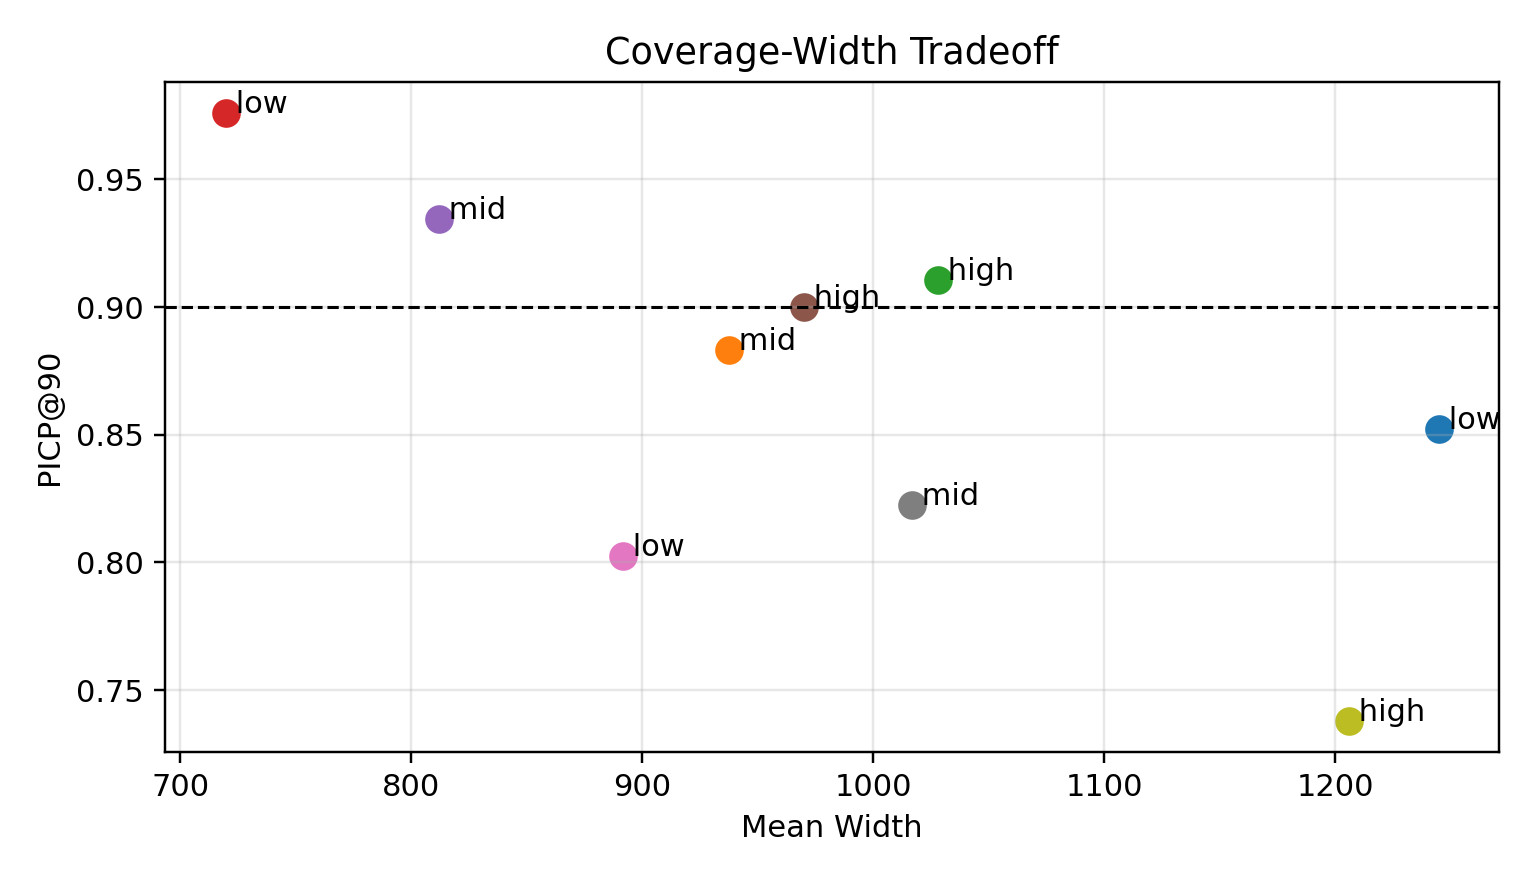
\includegraphics[width=0.85\textwidth]{reports/publication/fig_coverage_width_tradeoff.png}
\caption{Coverage--width tradeoff under temporal extension.  As the
  certificate ages (horizontal axis), the coverage probability decreases
  while the interval width increases.  The half-life (vertical dashed
  line) marks the crossover point.}
\label{fig:temporal-evidence}
\end{figure}

\subsection{What This Chapter Does Not Prove}

\begin{enumerate}
  \item The certificate validity horizon is a \emph{lower bound} on
    the true safe horizon; the actual safe horizon may be longer
    because drift is typically sub-maximal.
  \item The half-life corollary assumes sub-Gaussian drift; heavy-tailed
    drift distributions would require a different tail bound and would
    yield a shorter half-life.
  \item The graceful degradation dominance result compares to an
    \emph{uncontrolled} baseline.  A more sophisticated adaptive
    controller that is not quality-ignorant but uses a different
    inflation rule might also achieve zero violations with lower
    revenue loss.
  \item The safe-budget monotonicity holds only during the landing
    phase; during normal operation, the budget fluctuates with $w_t$.
  \item Multi-asset (fleet) temporal certificates are not covered here;
    compositional temporal extension is deferred to
    Chapter~\ref{ch:compositional-safety-fleets}.
\end{enumerate}

\subsection{Chapter Summary}

This chapter extends the ORIUS safety guarantee from per-step claims
to temporal and behavioral horizons.  Three temporal results---certificate
validity horizon (Theorem~\ref{thm:cert-horizon}), expiration bound
(Theorem~\ref{thm:cert-expiration}), and half-life corollary
(Corollary~\ref{cor:half-life})---quantify how long a safety certificate
remains valid after issuance.  Three behavioral results---fallback
existence (Theorem~\ref{thm:fallback-existence}), graceful degradation
dominance (Theorem~\ref{thm:graceful-dominance}), and safe-budget
monotonicity (Proposition~\ref{prop:budget-monotonicity})---formalise
the landing protocol and prove it is strictly safer than uncontrolled
dispatch.  Together, these extensions complete the theorem ladder
initiated in Chapter~\ref{ch:theorem-oasg}.
